\documentclass[]{mini}
\usepackage[utf8]{inputenc}
\usepackage{pdfpages}
\usepackage{mathtools}
\usepackage{mathrsfs}
%\usepackage{subfigure}
\usepackage{subcaption}
\usepackage{wrapfig,booktabs}
\usepackage{tikz}
\usepackage{float}
\usepackage{marginnote}
%\usepackage{pdflscape}
\usepackage{geometry}
\setlength{\marginparwidth}{1.8cm}
%\usepackage{mathmode}
% % % % % % % % % % % % % % % % % % % % % % %
\usepackage{lmodern}
\usepackage{amsmath}
\usepackage{amsfonts}
\usepackage{amssymb}
\usepackage{ifxetex,ifluatex}
\usepackage{fixltx2e} % provides \textsubscript
\ifnum 0\ifxetex 1\fi\ifluatex 1\fi=0 % if pdftex
  \usepackage[T1]{fontenc}
  \usepackage[utf8]{inputenc}
\else % if luatex or xelatex
  \ifxetex
    \usepackage{mathspec}
    \usepackage{xltxtra,xunicode}
  \else
    \usepackage{fontspec}
  \fi
  \defaultfontfeatures{Mapping=tex-text,Scale=MatchLowercase}
  \newcommand{\euro}{€}
\fi
% use upquote if available, for straight quotes in verbatim environments
\usepackage{color}
\usepackage{fancyvrb}
\newcommand{\VerbBar}{|}
\newcommand{\VERB}{\Verb[commandchars=\\\{\}]}
\DefineVerbatimEnvironment{Highlighting}{Verbatim}{commandchars=\\\{\}}
% Add ',fontsize=\small' for more characters per line
\usepackage{framed}
\definecolor{shadecolor}{RGB}{248,248,248}
\newenvironment{Shaded}{}{}
\newcommand{\KeywordTok}[1]{\textcolor[rgb]{0.13,0.29,0.53}{\textbf{{#1}}}}
\newcommand{\DataTypeTok}[1]{\textcolor[rgb]{0.13,0.29,0.53}{{#1}}}
\newcommand{\DecValTok}[1]{\textcolor[rgb]{0.00,0.00,0.81}{{#1}}}
\newcommand{\BaseNTok}[1]{\textcolor[rgb]{0.00,0.00,0.81}{{#1}}}
\newcommand{\FloatTok}[1]{\textcolor[rgb]{0.00,0.00,0.81}{{#1}}}
\newcommand{\CharTok}[1]{\textcolor[rgb]{0.31,0.60,0.02}{{#1}}}
\newcommand{\StringTok}[1]{\textcolor[rgb]{0.31,0.60,0.02}{{#1}}}
\newcommand{\CommentTok}[1]{\textcolor[rgb]{0.56,0.35,0.01}{\textit{{#1}}}}
\newcommand{\OtherTok}[1]{\textcolor[rgb]{0.56,0.35,0.01}{{#1}}}
\newcommand{\AlertTok}[1]{\textcolor[rgb]{0.94,0.16,0.16}{{#1}}}
\newcommand{\FunctionTok}[1]{\textcolor[rgb]{0.00,0.00,0.00}{{#1}}}
\newcommand{\RegionMarkerTok}[1]{{#1}}
\newcommand{\ErrorTok}[1]{\textbf{{#1}}}
\newcommand{\NormalTok}[1]{{#1}}
%\ifxetex
%  \usepackage[setpagesize=false, % page size defined by xetex
%              unicode=false, % unicode breaks when used with xetex
%              xetex]{hyperref}
%\else
%  \usepackage[unicode=true]{hyperref}
%\fi
%\hypersetup{breaklinks=true,
%            bookmarks=true,
%            colorlinks=true,
%            citecolor=blue,
%            urlcolor=blue,
%            linkcolor=magenta,
%            pdfborder={0 0 0}}
\urlstyle{same}  % don't use monospace font for urls
\setlength{\parindent}{0pt}
\setlength{\parskip}{6pt plus 2pt minus 1pt}
\setlength{\emergencystretch}{3em}  % prevent overfull lines
% % % % % % % % % % % % % % % % % % % % % % % % % % %
\hypersetup{breaklinks=true,
            bookmarks=true,
            colorlinks=true,
            citecolor=blue,
            urlcolor=blue,
            linkcolor=magenta,
            pdfborder={0 0 0}}
\usepackage{url}
\usepackage[sort]{natbib}
%------------------------------------------------------------------------------%
\title{Estymacja w modelu Coxa metodą~stochastycznego~spadku~gradientu z~przykładami~zastosowań~w~analizie~danych z~The~Cancer~Genome~Atlas}
\titleaux{Stochastic gradient descent method in~Cox~models~with~applications to The~Cancer~Genome~Atlas~data}
\author{Marcin Piotr Kosiński}
\supervisor{\text{dr hab. inż Przemysław Biecek, prof. nadzw.}}
\type{magisters}
\discipline{matematyka}
\specialty{Statystyka Matematyczna i Analiza Danych}
\monthyear{grudzień 2015}
\date{\today}
\album{265361}
%------------------------------------------------------------------------------%
\begin{document}
%\bibliographystyle{authordate1}
%\bibliographystyle{authordate}
\bibliographystyle{apalike}
%\setcitestyle{numbers}
\setcitestyle{authoryear}
%\setcitestyle{authoryear, open={},close={}}

\maketitle

\begin{center}
\textbf{Streszczenie}
\end{center}

Praca przedstawia zastosowanie algorytmu numerycznej optymalizacji metodą stochastycznego spadku gradientu do wyznaczenia współczynników w modelu proporcjonalnych hazardów Coxa, opartych na analitycznej metodzie wyznaczania estymatorów metodą największej wiarogodności. Zaprezentowano zastosowanie tego algorytmu do napływających danych, wyliczając kolejne kroki optymalizacji w algorytmie w oparciu o częściową funkcję log-wiarogodności, konstruowaną na bazie obecnie zaobserwowanego podzbioru obserwacji. Zaprezentowane podejście jest nowatorskie. Wcześniej nie wykorzystywano tego podejścia w modelu Coxa.

Opisano matematyczne własności estymatorów największej wiarogodności, przedstawiono model Coxa wraz z najważniejszymi jego cechami, scharakteryzowano algorytm stochastycznego spadku gradientu oraz jego różnice w stosunku go algorytmów spadku gradientu, zaimplementowano algorytm numerycznej optymalizacji metodą stochastycznego spadku gradientu do wyznaczenia współczynników w modelu proporcjonalnych hazardów Coxa oraz przeprowadzono analizę rzeczywistych danych genomicznych, wykorzystując stworzony algorytm. Pracę wzbogacono o symulacje zbieżności procesu optymalizacji funkcji log-wiarogodności w~modelu regresji logistycznej, które przygotowane zostały dla algorytmów spadku gradientu rzędu I, spadku gradientu rzędu II oraz stochastycznego spadku gradientu rzędu I. Dzięki temu możliwe było zobrazowanie różnic w opisywanych metodach numerycznej optymalizacji. Dodatkowo przeprowadzono symulacje przy sztucznie wygenerowanych danych do analizy przeżycia z rozkładu Weibulla, pozwalające zobrazować proces zbieżności nowo wprowadzonego algorytmu numerycznej optymalizacji metodą stochastycznego spadku gradientu do wyznaczenia współczynników w modelu proporcjonalnych hazardów Coxa.

Proces estymacji w modelu proporcjonalnych hazardów Coxa, z wykorzystaniem metody stochastycznego spadku gradientu, w sytuacji napływających danych wygląda na stabilny i zbiega w okolice bliskie do teoretycznego optimum, niekiedy nawet już po jednej epoce. Przy dobrze dobranych parametrach optymalizacji, proces może być z powodzeniem wykorzystywany do znajdowania współczynników modelu. Kluczowym momentem, mającym wpływ na powodzenie optymalizacji, jest wybór ciągu odpowiedzialnego za dobór długości kroków, więc zaleca się symulacje badające różne ciągi oraz wybranie tego ciągu, który w~większości przypadków daje stabilne, jednorodne współczynniki, maksymalizujące częściową funkcję log-wiarogodności, konstruowaną w oparciu o zbiór testowy. 

Do analizy genomicznej wykorzystano środowisko statystyczne $\mathcal{R}$, a wykorzystane funkcje, zaimplementowane algorytmy i przygotowaną dokumentację do stworzonego w trakcie pracy pakietu \texttt{coxphSGD} zamieszczono w Dodatku \ref{docCoxSGD}. W analizie badano wpływ występowania mutacji w poszczególnych genach na czas przeżycia pacjentów, dla których dane kliniczne i~dane o występowaniu mutacji zaczerpnięto z badania \textit{The Cancer Genome Atlas}. Zaprezentowano skuteczność badanego modelu oraz wskazano geny odpowiedzialne za zwiększenie ryzyka zgonu w~trakcie choroby nowotworowej. \ \\
\begin{center}
\textbf{Słowa kluczowe} 
\end{center}
model proporcjonalnych hazardów Coxa, stochastyczny spadek gradientu, estymacja metodą największej wiarogodności, częściowa funkcja wiarogodności, analiza przeżycia, pakiet statystyczny $\mathcal{R}$, napływające dane, nowotworzenie, \textit{The~Cancer~Genome~Atlas} \ \\
\begin{center}
\textbf{Tytuł pracy w języku angielskim} \\ \ \\ \vspace{-10pt}
Stochastic gradient descent method in Cox models with applications to \\ The~Cancer~Genome~Atlas~data.
\end{center}



\tableofcontents
%\listoffigures

\chapter*{Wprowadzenie}


+++
Analiza przeżycia.
+++

Najbardziej charakterystyczną cechą typowych danych, jakimi posługuje się w analizie przeżycia, jest obecność obiektów, w których końcowe zdarzenie nastąpiło (wówczas ma się do czynienia z obserwacjami \textit{kompletnymi}), oraz obiektów, w których to zdarzenie (jeszcze) nie nastąpiło (obserwacja \textit{ucięta}). Ta specyficzna postać danych statystycznych doprowadziła do powstania specjalnych metod stosowanych tylko w analizie czasu trwania zjawisk. Jednym z takich modeli jest model proporcjonalnych hazardów Coxa. Jak podaje \cite{assel}, model proporcjonalnych hazardów Coxa jest jednym z najszerzej stosowanych modeli w onkologicznych publikacjach naukowych, ale także jedną z najmniej rozumianych metod statystycznych. Wynika to z łatwego dostępu do pakietów statystycznych zawierających programy do analizy przeżyć, modeli regresji i analiz wielowariantowych, ale prawie nigdy nie zawierających dobrego opisu podstawowych zasad działania modelu Coxa. Dostarczają one wyłącznie instrukcje, jak wprowadzić dane i uruchomić odpowiednie procedury w celu uzyskania wyniku. Poniższy praca zawiera pełny opis metodologii modelu proporcjonalnych hazardów Coxa, w tym wyjaśnienie najważniejszych pojęć. 


++++++++


\chapter*{Podstawy modelu statystycznego}

W pracy zakłada się znajomość podstaw statystyki matematycznej. Aby ujednolicić oznaczenia w niniejszym rozdziale wprowadzona została klasyczna nomenklatura oparta~o~\cite{niemiro}.

\begin{definition} 
\textbf{Model statystyczny} określamy przez podanie rodziny $\{ \mathbb P_{\theta}:\theta\in\Theta\} $ rozkładów prawdopodobieństwa na przestrzeni próbkowej $\Omega$ oraz zmiennej losowej $X : \Omega \rightarrow \mathcal{X}$, którą traktujemy jako obserwację. Zbiór $\mathcal{X}$ nazywamy przestrzenią obserwacji, zaś $\Theta$ nazywamy przestrzenią parametrów. \\
\end{definition}
Symbol $\theta$ jest nieznanym parametrem opisującym rozkład badanego zjawiska. Może być jednowymiarowy lub wielowymiarowy. Determinując opis zjawiska poprzez podanie parametru $\theta$, jednoznacznie wyznaczany jest rozkład rozważanego zjawiska spośród całej rodziny rozkładów prawdopodobieństwa $\{ \mathbb P_{\theta}:\theta\in\Theta\}$, co umożliwia określenie prawdziwości tezy.
\par
Zakłada się, że przestrzeń próbkowa $\Omega$ jest wyposażona w $\sigma$-ciało $\mathcal{F}$. Wtedy:
\begin{definition}
\textbf{Przestrzenią statystyczną} nazywa się trójkę $(\mathcal{X},\mathcal{F},\{\mathbb P_{\theta}:\theta\in\Theta\})$.
\end{definition}
Wprowadzenie $\sigma$-ciała $\mathcal{F}$ sprawia, że przestrzeń statystyczna staje się przestrzenią mierzalną, a więc można na niej określić rodzinę miar $\{ \mathbb P_{\theta}:\theta\in\Theta\} $, dzięki której da się ustalić prawdopodobieństwa$  $ zajścia wszystkich zjawisk w rozważanej teorii.

W celu budowania niezbędnych pojęć potrzebna jest również definicja losowej próby statystycznej, zazwyczaj nazywanej \textit{próbką}.

\begin{definition}
 \textbf{Losową próba statystyczną} nazywamy zbiór obserwacji statystycznych wylosowanych z populacji, które są realizacjami ciągu zmiennych losowych o rozkładzie takim jak rozkład populacji.
 \end{definition}

\chapter{Estymacja metodą największej wiarogodności}
\begin{flushright}
\textit{The making of maximum likelihood was one of \\
the most important developments in 20th century statistics. \\
It was the work of one man but it was no simple process (...). \\
John Aldrich o R. A. Fisher'ze
}
\end{flushright}

\section{Estymacja}

Estymacja to dział wnioskowania statystycznego będący zbiorem metod pozwalających na uogólnianie wyników badania próby losowej na nieznaną postać i parametry rozkładu zmiennej losowej całej populacji oraz szacowanie błędów wynikających z tego uogólnienia \cite{wiki1}.

W statystyce parametrycznej zakłada się, że rozkład prawdopodobieństwa
opisujący doświadczenie należy do rodziny $\{\mathbb{P}_{\theta} : \theta \in \Theta\}$, ale nie zna się
parametru $\theta$. Można go jednak szacować dzięki estymatorom opartym na statystykach.

\begin{definition}
\textbf{Statystyka}, dla $X=(X_1,\dots,X_n)$, to odwzorowanie mierzalne $T: \mathcal{X} \rightarrow \mathcal{R}.$
\end{definition}

\begin{definition}
\textbf{Estymatorem} parametru $\theta$ nazywamy dowolną statystykę
$T = T(X)$, gdzie $X$ to próba z badanego rozkładu, o wartościach w zbiorze $\Theta$. 
\end{definition}

Interpretuje się $T$ jako przybliżenie $\theta$ i często estymator $\theta$ oznacza symbolem $\hat{\theta}$. Niekiedy w kręgu zainteresowań jest również estymacja $g(\theta)$, gdzie $g$ to ustalona funkcja.

Pewne estymatory mające odpowiednie własności są preferowane nad inne ze względu na większą precyzję bądź ufność oszacowania danego estymatora. Poniżej przedstawione są 2 ważne definicje związane z jakością estymatorów \cite{niemiro}, gdy rozmiar próbki $X_1, \dots , X_n$ jest duży. Mówi się wtedy o własnościach asymptotycznych estymatorów, które z matematycznego punktu widzenia, są twierdzeniami
granicznymi, w których $n$ dąży do nieskończoności. Dzięki tym twierdzeniom możliwe jest opisane w przybliżeniu zachowania estymatorów dla dostatecznie dużych próbek. Niestety, teoria asymptotyczna nie dostarcza informacji o tym, jak duża powinna być próbka, żeby przybliżenie było dostatecznie dobre.

\begin{definition}
Estymator $\hat{g}(X_1, \dots , X_n)$ wielkości $g(\theta)$ jest \textbf{nieobciążony}, \text{jeśli dla każdego $n$} 
$$\mathbb{E}\hat{g}(X_1, \dots , X_n) = g(\theta).$$

\end{definition}

\begin{definition}
Estymator $\hat{g}(X_1, \dots , X_n)$ wielkości $g(\theta)$ jest \textbf{zgodny},
jeśli dla każdego $\theta \in \Theta$
$$ \lim\limits_{n \rightarrow \infty} \mathbb{P}_{\theta}(|\hat{g}(X_1,\dots,X_n) -g(\theta)| \leq \varepsilon ) = 1,$$
dla każdego $\varepsilon > 0.$
\end{definition}

\begin{definition}
Estymator $\hat{g}(X_1, \dots , X_n)$ wielkości $g(\theta)$ jest \textbf{mocno zgodny},
jeśli %dla każdego $\theta \in \Theta$
$$\mathbb{P}_{\theta}\Big(\lim\limits_{n \rightarrow \infty}\hat{g}(X_1,\dots,X_n)=g(\theta) \Big) = 1.$$
\end{definition}


Zgodność (mocna zgodność) znaczy tyle, że
$$\hat{g}(X_1, \dots , X_n) \rightarrow g(\theta), \ \ \ \ \ (n \rightarrow \infty)$$
według prawdopodobieństwa (prawie na pewno). Interpretacja jest taka: estymator jest uznany za
zgodny, jeśli zmierza do estymowanej wielkości przy nieograniczonym powiększaniu badanej próbki.

Jednak zgodność (nawet w mocnym sensie) nie jest specjalnie satysfakcjonującą własnością estymatora,
a zaledwie minimalnym żądaniem, które powinien spełniać każdy przyzwoity estymator. Dlatego od niektórych estymatorów żąda się silniejszych właściwości, takich jak asymptotyczna normalność.

\begin{definition}
\marginnote{\small{$\overset{d}{\rightarrow}$ oznacza zbieżność wg rozkładu.}}[1cm]
Estymator $\hat{g}(X_1, \dots , X_n)$ wielkości $g(\theta)$ jest \textbf{asymptotycznie normalny}, jeśli dla każdego $\theta \in \Theta$ istnieje funkcja $\sigma^2(\theta)$, zwana asymptotyczną wariancją, taka że
$$\sqrt{n}(\hat{g}(X_1,\dots,X_n) -g(\theta))  \overset{d}{\rightarrow} \mathcal{N}(0, \sigma^2(\theta)), \ \ \ (n \rightarrow \infty).$$
\end{definition}


Oznacza to, że rozkład prawdopodobieństwa statystyki $\hat{g}(X_1,\dots,X_n)$ jest dla dużych $n$ zbliżony do rozkładu $$\mathcal{N}\Big(g(\theta), \dfrac{\sigma^2(\theta)}{n}\Big).$$ Inaczej mówiąc, estymator jest asymptotycznie normalny, gdy: 
$$\lim\limits_{n \rightarrow \infty} \mathbb{P}_{\theta} \Big(\dfrac{\sqrt{n}}{\sigma(\theta)}(\hat{g}(X_1,\dots,X_n) -g(\theta) \leq a \Big) = \Phi(a),$$
gdzie $\Phi(x)$ to dystrybuanta standardowego rozkładu normalnego $\mathcal{N}(0,1)$.

Asymptotyczna normalność mówi, że estymator nie tylko zbiega do nieznanego parametru, ale również że zbiega wystarczająco szybko, jak $\frac{1}{\sqrt{n}}$, czyli, że 
$$\mathbb{P}_{\theta} \Big(\dfrac{\sqrt{n}}{\sigma(\theta)}(\hat{g}(X_1,\dots,X_n) -g(\theta) \leq a \Big) - \Phi(a) = f(n) \in \eth(\frac{1}{\sqrt{n}}) . $$ 

Jeśli estymator jest asymptotycznie normalny, to jest zgodny, choć nie musi
być \textit{\text{mocno zgodny}}.

W dalszej części tego rozdziału zostanie wprowadzone pojęcie estymatora największej wiarogodności oraz zostaną udowodnione dla niego jego właściwości, co utwierdzi w przekonaniu, że metoda największej wiarogodności, przy odpowiednich założeniach, jest metodą konstrukcji rozsądnych estymatorów.

\newpage 

\section{Metoda największej wiarogodności}

Metodę największej wiarogodności wprowadził R. A. Fisher w 1922 r. \cite{fisher2}, dla której po raz pierwszy procedurę numeryczną zaproponował już w 1912 r. \cite{fisher1}. O burzliwym procesie powstawania metody, o zmianach w jej uzasadnieniu, o koncepcjach, które powstały w obrębie tej metody takich jak parametr, statystyka, wiarogodność, dostateczność czy efektywność oraz o podejściach, które Fisher odrzucił tworząc podstawy pod nową teorię można przeczytać w~obszernej pracy dokumentalnej \cite{aldrich1}. 

Metoda ta, jako alternatywa dla metody najmniejszych kwadratów \cite{legendre1}, \cite{gauss1}, była rozwijana i szeroko stosowana później przez wielu statystyków i wciąż znajduje obszerne zastosowania w wielu obszarach estymacji statystycznej, np. \cite{hutch1}, \cite{kenward1}, \cite{millar1}.

Aby zdefiniować estymator oparty o metodę największej wiarogodności, należy najpierw wprowadzić pojęcie funkcji wiarogodności.

\begin{definition}
\textbf{Funkcją wiarogodności} nazywamy funkcję $L : \Theta \rightarrow \mathbb{R}$ daną wzorem $$ L(\theta) =L(\theta;x_1, \dots , x_n) = f(\theta; x_1, \dots , x_n),$$
którą rozważamy jako funkcję parametru $\theta$ przy ustalonych wartościach obserwacji $x_1, \dots , x_n$, gdzie $$ f(\theta; x_1, \dots , x_n) = \begin{dcases*}
 \mathbb{P}_{\theta}( X_1 = x_1, \dots , X_n = x_n), & dla rozkładów dyskretnych,  \\
 f_{\theta}(x_1, \dots , x_n), & dla rozkładów absolutnie ciągłych.
\end{dcases*}$$

\end{definition}

Oznacza to, że wiarogodność jest właściwie tym samym, co gęstość prawdopodobieństwa,
ale rozważana jako funkcja parametru $\theta$, przy ustalonych wartościach obserwacji
$x = X(\omega)$.


\begin{definition}
\textbf{Estymatorem największej wiarogodności} parametru $\theta$, oznaczanym ENW($\theta$), nazywamy wartość parametru, w której funkcja
wiarogodności przyjmuje supremum $$L(\hat{\theta}) = \sup_{\theta \in \Theta} L(\theta).$$

\end{definition}

Ponieważ takie supremum może nie istnieć, niektóre pozycje w literaturze, w definicji estymatora największej wiarogodności, supremum zastępują wartością największą \cite{rydl1},~\cite{sfu1},~\cite{mit0}.

\section{Asymptotyczne własności estymatora największej wiarogodności}

W tym podrozdziale zostanie wykazane, że estymator największej wiarygodności jest
\begin{enumerate}
\item[i)] zgodny,
\item[ii)] asymptotycznie normalny,
\item[iii)] asymptotycznie nieobciążony.
\end{enumerate}

Asymptotyczna nieobciążoność wynika z asymptotycznej normalności. \newline
Dowody w tym rozdziale są znane w literaturze i opierają się o \cite{mit1} i \cite{sfu1}.



\subsection{Zgodność estymatora największej wiarogodności}

Chcąc wykazać zgodność estymatora największej wiarogodności \textit{przy pewnych warunkach regularności}
przydatna będzie poniższa definicja i następujący Lemat.
\begin{definition}
\textbf{Funkcja log-wiarogodności} to funkcja spełniająca równanie
$$\ell(\theta) = \log(L(\theta)),$$
gdzie przyjmuje się $\ell(\theta) = -\infty$ jeśli $L(\theta) = 0$.
\end{definition}

\begin{lemma}\label{l:pierwszy}
Gdy $\theta_0$ to prawdziwe maksimum funkcji wiarogodności, to dla każdego \text{$\theta \in \Theta$}
$$\mathbb{E}_{\theta_0}\ell(\theta) \leq \mathbb{E}_{\theta_0}\ell(\theta_0).$$
\end{lemma}

\begin{proof}
Rozważając różnicę, przy założeniu ciągłości rozkładu:
\begin{equation*}
\begin{split}
\mathbb{E}_{\theta_0}\ell(\theta) - \mathbb{E}_{\theta_0}\ell(\theta_0) & = \mathbb{E}_{\theta_0}(\ell(\theta) - \ell(\theta_0) ) = \mathbb{E}_{\theta_0}(\log f(\theta; X) - \log f(\theta_0; X)) \\
 & = \mathbb{E}_{\theta_0}\log\dfrac{f(\theta; X)}{f(\theta_0; X)},
\end{split}
\end{equation*}
i pamiętając o tym, że $\log t \leq t - 1$, można dojść do
\marginnote{\tiny{$\mathbb{E}_{\theta_0}$ oznacza wartość oczekiwaną względem rozkładu parametryzowanego przez $\theta_0$.}}[0.5cm]
\begin{equation*}
\begin{split}
\mathbb{E}_{\theta_0}\log\dfrac{f(\theta; X)}{f(\theta_0; X)} & \leq \mathbb{E}_{\theta_0}\Big(\dfrac{f(\theta; X)}{f(\theta_0; X)} - 1 \Big) = \int \Big(\dfrac{f(\theta; x)}{f(\theta_0; x)} - 1 \Big) f(\theta_0;x) dx \\ 
& = \int f(\theta;x)dx - \int f(\theta_0;x)dx = 1-1 =0.
\end{split}
\end{equation*}
Obie całki równają się 1 jako, że są całkami z funkcji gęstości, zaś równość w nierówności zachodzi tylko wtedy, gdy  $\mathbb{P}_{\theta}=\mathbb{P}_{\theta_0}$.
\end{proof}

Dzięki temu wynikowi możliwe jest udowodnienie poniższego Twierdzenia.

\begin{theorem}
Pod pewnymi \textbf{warunkami regularności} nałożonymi na rodzinę rozkładów prawdopodobieństwa, estymator największej wiarogodności $ENW(\theta)$ jest zgodny, tzn. 
$$ENW(\theta) \rightarrow \theta \ \ \text{dla } \ \ n \rightarrow \infty.$$
\end{theorem}
\begin{proof}
\ \\
1) Z definicji w $ENW(\theta)$ przyjmowana jest wartość największa funkcji $L(\theta)$, a więc tym bardziej funkcji $ \ell(\theta) = \log L(\theta)$ oraz funkcji $$ \ell_n(\theta) = \frac{1}{n}\ell(\theta) = \frac{1}{n}\log L(\theta) = \frac{1}{n}\sum\limits_{i=1}^{n}\log f(\theta;X_i)$$ (zakładając ciągłość rozkładu i niezależność $X_1,\dots,X_n$), gdyż ekstremum jest niezmiennicze ze względu na monotoniczną transformację i liniowe przekształcenie jakim jest dzielenie.

2) Z Lematu \ref{l:pierwszy} wynika, że $\theta_0$ maksymalizuje $\mathbb{E}_{\theta_0}\ell(\theta)$.

3) Z Prawa Wielkich Liczb, które jest spełnione gdy założy się, że $X_i$ to realizacje ciągu zmiennych losowych o skończonych wartościach oczekiwanych, wynika, że $$ \ell_n(\theta) = \frac{1}{n}\sum\limits_{i=1}^{n}\log f(\theta;X_i) \rightarrow \mathbb{E}_{\theta_0}\ell(\theta),$$ co ostatecznie oznacza, że $ENW(\theta)$ jest zgodny.
\end{proof}

\newpage
\subsection{Asymptotyczna normalność estymatora największej wiarygodności}


Fisher w swojej karierze wprowadził wiele pożytecznych pojęć stosowanych do dziś. Jednym z nich jest Informacja Fishera, która zostanie wykorzystana w dowodzie asymptotycznej normalności estymatora największej wiarogodności.

\begin{definition}
Niech $X$ będzie zmienną losową o gęstości $f_{\theta}$, zależnej od jednowymiarowego parametru $\theta \in \Theta \subset \mathbb{R}$. \textbf{Informacją Fishera} zawartą w obserwacji $X$ nazywa się funkcję
\begin{equation}\label{wzor:fish}
\mathcal{I}(\theta) = \mathbb{E}_{\theta}(\ell'(\theta;X))^2 = \mathbb{E}_{\theta}\Big(\frac{\partial}{\partial\theta}\log f_{\theta}(X) \Big)^2,
\end{equation}
gdzie odpowiednio
\begin{align*}
\mathcal{I}(\theta) = & \int \Big(\frac{\partial}{\partial\theta}\log f_{\theta}(x) \Big)^2 f_{\theta}(x)dx \ \text{\ \ \ \ \ dla zmiennej ciągłej;} \\
\mathcal{I}(\theta) = & \sum\limits_{x}^{ } \Big(\frac{\partial}{\partial\theta}\log f_{\theta}(x) \Big)^2 \mathbb{P}_{\theta}(X=x) \ \text{dla zmiennej dyskretnej}.
\end{align*}
\end{definition}

W dowodzie asymptotycznej normalności estymatora największej wiarogodności kluczowymi założeniami są poniższe warunki regularności. Rodzina gęstości musi być dostatecznie regularna aby pewne kroki rachunkowe w dalszych rozumowaniach były
poprawne.

\begin{definition}\label{def:regur}
\textbf{Warunki regularności.}
\end{definition}
\begin{itemize}
\item[$i)$] Informacja Fishera jest dobrze określona. Zakłada się, że $\Theta$ jest przedziałem
otwartym, istnieje pochodna $\frac{\partial}{\partial\theta}\log f_{\theta}$, całka/suma we wzorze
(\ref{wzor:fish}) jest bezwzględnie zbieżna (po obłożeniu funkcji podcałkowej modułem całka istnieje i jest skończona) i $0 < \mathcal{I}(\theta) < \infty$.
\item[$ii)$] Wszystkie gęstości $f_\theta$ mają jeden nośnik, tzn. zbiór $\{x \in X : f_\theta(x) > 0\}$ nie zależy~od~$\theta$.
\item[$iii)$] Można przenosić pochodną przed znak całki, czyli zamienić kolejność
operacji różniczkowania $\frac{\partial}{\partial\theta}$ i całkowania $\int \dots dx$.
\end{itemize}

Wprowadzając takie założenia, otrzymano przydatne właściwości~Informacji~Fishera.

\begin{proposition}\label{prop:warunki}
Jeśli spełnione są warunki regularności (\ref{def:regur}) to:
\begin{align*}
(i) \ & \ \mathbb{E}_\theta\frac{\partial}{\partial\theta}\log f_{\theta}(x) = 0, \\
(ii) \ & \ \mathcal{I}(\theta) = \mathbb{V}ar_{\theta}\Big(\frac{\partial}{\partial\theta}\log f_{\theta}(X) \Big), \\
(iii) \ & \ \mathcal{I}(\theta) = -\mathbb{E}_{\theta}\Big(\frac{\partial^2}{\partial\theta^2}\log f_\theta(X) \Big).
\end{align*}
\end{proposition}

Dowód tego stwierdzenia można znaleźć w \cite{niemiro}.

\newpage
Patrząc na postać pochodnej funkcji log-wiarogodności
$$\ell'(\theta_0;X) = (\log f(\theta_0;X))' = \dfrac{f'(\theta_0;X)}{f(\theta_0;X)},$$
można wywnioskować, że nieformalnie interpretacja Informacji Fishera jest miarą tego jak szybko zmieni się funkcja gęstości jeśli delikatnie zmieni się parametr $\theta$ w okolicach $\theta_0$. Biorąc kwadrat i wartość oczekiwaną, innymi słowy uśredniając po $X$, otrzymuje się uśrednioną wersję tej miary. Jeżeli Informacja Fishera jest duża, oznacza to, że gęstość zmieni się szybko gdyby poruszyć parametr $\theta_0$, co innymi słowy oznacza, że gęstość z parametrem $\theta_0$ jest \textit{znacząco inna} i \textit{może zostać łatwo odróżniona} od gęstości z parametrami nie tak bliskimi $\theta_0$. Oznacza to, że możliwa estymacja $\theta_0$ oparta o takie dane jest dobra. Z drugiej strony, jeżeli Informacja Fishera jest mała, oznacza to, że gęstość dla $\theta_0$ jest bardzo podobna do gęstości z parametrami nie tak bliski do $\theta_0$, a co za tym idzie, dużo ciężej będzie odróżnić tę gęstość, czyli estymacja będzie słabsza.

Dzięki pojęciu Informacji Fishera i warunkom regularności, możliwe jest udowodnienie poniższego Twierdzenia.

\begin{theorem}
Pod pewnymi \textbf{warunkami regularności} nałożonymi na rodzinę rozkładów prawdopodobieństwa, estymator największej wiarogodności jest asymptotycznie normalny, 
$$ \sqrt{n}(ENW(\theta) - \theta_0) \rightarrow \mathcal{N}\Big(0, \dfrac{1}{\mathcal{I}(\theta_0)}\Big).$$
\end{theorem}

Z Twierdzenia widać, że im większa Informacja Fishera tym mniejsza asymptotyczna wariancja estymatora prawdziwego parametru $\theta_0$.

\begin{proof}
Ponieważ $ENW(\theta)$ maksymalizuje $\ell_n(\theta) = \frac{1}{n}\sum\limits_{i=1}^{n}\log f(\theta;X)$, to $\ell'_n(\theta)=0$. \\ Dalej, korzystając z Twierdzenia o Wartości Średniej:
$$\dfrac{g(a)-g(b)}{a-b} = g'(c) \ \text{albo} \ g(a)=g(b)+g'(c)(a-b), \ \text{dla} \ c \in [a,b],$$
gdzie $g(\theta) = \ell'_n(\theta), a = ENW(\theta), b = \theta_0$, można zapisać równość
$$ 0 = \ell'_n(ENW(\theta)) = \ell'_n(\theta_0) + \ell''_n(\theta_1)(ENW(\theta)-\theta_0), \ \text{dla} \ \theta_1 \in [ENW(\theta),\theta_0],$$ 
a z niej przejść do postaci 
\begin{equation}\label{dowod1}
\sqrt{n}(ENW(\theta)-\theta_0) = - \dfrac{\sqrt{n}\ell'_n(\theta_0)}{\ell''_n(\theta_1)}.
\end{equation}
Z Lematu (\ref{l:pierwszy}) wynika, że $\theta_0$ maksymalizuje $\mathbb{E}_{\theta_0}\ell(\theta_0)$ czyli
\begin{equation}\label{row:maksymalizator}
\mathbb{E}_{\theta_0}\ell'(\theta_0) = 0,
\end{equation}
a to można wstawić do licznika w równaniu (\ref{dowod1})
\begin{equation}\label{dowod2}
\begin{split}
\sqrt{n}\ell'_n(\theta_0) & = \sqrt{n}\Big(\frac{1}{n}\sum\limits_{i=1}^{n}\ell'(\theta_0) - 0\Big) \\
& = \sqrt{n}\Big(\frac{1}{n}\sum\limits_{i=1}^{n}\ell'(\theta_0) - \mathbb{E}_{\theta_0}\ell'(\theta_0)\Big) \rightarrow \mathcal{N}\Big(0, \mathbb{V}ar_{\theta_0}(\ell'(\theta_0))\Big),
\end{split}
\end{equation}
gdzie zbieżność wynika z Centralnego Twierdzenia Granicznego. 
\newpage
Następnie można rozważyć mianownik w równaniu (\ref{dowod1}). Dla wszystkich $\theta$ wynika
$$\ell''(\theta) = \frac{1}{n}\sum\limits_{i=1}^{n}\ell''(\theta) \rightarrow \mathbb{E}_{\theta_0}\ell''(\theta)$$
z Prawa Wielkich Liczb. \\ \ \\ Dodatkowo, ponieważ $\theta_1 \in [ENW(\theta),\theta_0]$ a $ENW(\theta)$ jest zgodny (poprzedni podrozdział), to ponieważ $ENW(\theta) \rightarrow \theta_0$, to też $\theta_1 \rightarrow \theta_0$, a wtedy
$$\ell''_n(\theta_1) \rightarrow \mathbb{E}_{\theta_0}\ell''(\theta_0) = -\mathcal{I}(\theta_0)$$
z punktu $(iii)$ ze Stwierdzenia (\ref{prop:warunki}).\\ \ \\ Wtedy prawa strona równania (\ref{dowod1}), dzięki (\ref{dowod2})
$$- \dfrac{\sqrt{n}\ell'_n(\theta_0)}{\ell''_n(\theta_1)} \overset{d}{\rightarrow} \mathcal{N}\Big(0,\dfrac{\mathbb{V}ar_{\theta_0}(\ell'(\theta_0))}{(\mathcal{I}(\theta_0))^2} \Big).$$
Ostatecznie wariancja
$$\mathbb{V}ar_{\theta_0}(\ell'(\theta_0)) \overset{z \ def}{=} \mathbb{E}_{\theta_0}(\ell'(\theta_0))^2 - (\mathbb{E}_{\theta_0}\ell'(\theta_0))^2 = \mathcal{I}(\theta_0) - 0,$$
co wynika z definicji Informacji Fishera i (\ref{row:maksymalizator}).

\end{proof}
\chapter{Model Coxa}
\begin{flushright}
\textit{The proportion of my life that I spent working on the \\ 
proportional hazards model is, in fact, very small. I had an \\
 idea of how to solve it but I could not complete the \\
  argument and so it took me about four years on and off... \\
Sir David Cox, An interview with Sir David Cox, 2014.
}
\end{flushright}


W tym rozdziale zostanie przedstawiony model proporcjonalnych hazardów Coxa. Głównym celem tej pracy jest wykorzystanie, nietypowej w tym modelu, numerycznej metody estymacji współczynników metodą stochastycznego spadku gradientu. Więcej o estymacji metodą stochastycznego spadku gradientu napisane jest w rozdziale \ref{SGD}. Definicje i twierdzenia w tym rozdziale oparte są o \cite{cox}, \cite{ther} i \cite{assel}.

%\section{Nomenklatura i podstawy analizy przeżycia}

%Analiza przeżycia to zbiór metod statystycznych badających procesy, w których interesujący jest czas, jaki upłynie do (pierwszego) wystąpienia pewnego zdarzenia.

\section{Wprowadzenie do modelu Coxa i nomenklatura}

Model proporcjonalnych hazardów Coxa \cite{cox} jest obecnie najczęściej stosowaną procedurą do modelowania relacji pomiędzy zmiennymi objaśniającymi a przeżyciem lub innym cenzurowanym rezultatem. Model ten umożliwia analizę wpływu czynników prognostycznych na przeżycie. Sir David Cox opracował tego typu model dla tabeli przeżyć i zilustrował zastosowanie modelu dla przypadku
leukemii, ale model może być stosowany do obliczania
przeżyć w odniesieniu do wszystkich innych chorób, jak
w przypadku przeżyć w chorobach nowotworowych lub
kardiologicznych po transplantacji serca lub zawałach
serca \cite{norwe}. 

\begin{definition}
\textbf{Model Coxa} określa funkcję hazardu dla i-tej obserwacji $X_i$ jako
\begin{equation}
\lambda_i(t) = \lambda_0(t)e^{X_i(t)\beta},
\end{equation}
gdzie $\lambda_0$ to niesprecyzowana nieujemna funkcja nazywana \textit{bazowym hazardem}, a $\beta$ to wektor współczynników o rozmiarze $p$, co odpowiada liczbie zmiennych objaśniających w modelu.
\end{definition}

Wspomnianą funkcję hazardu definiuje się jak następuje:
\begin{definition}
\textbf{Funkcja hazardu} to funkcja, która wyraża się wzorem
\begin{equation}
\begin{align*}
\lambda_j(t) & =  \lim\limits_{h\rightarrow 0}\dfrac{\mathbb{P}(t \leq T^* \leq t +h | T^* \geq t)}{h} & \ \\
 \ & = \lim\limits_{h\rightarrow 0}\dfrac{\mathbb{P}(t \leq T^* \leq t +h )}{h}\cdot\frac{1}{  \mathbb{P}(T^* \geq t)} & \ \\ \ & = \lim\limits_{h\rightarrow 0} \frac{F_j(t+h) - F_j(t) }{h}\cdot\frac{1}{S_j(t)} & =  \frac{f_j(t)}{S_j(t)}.
 \end{align*}
\end{equation}
\end{definition}

W powyższej definicji $T^*$ oznacza czas do wystąpienia zdarzenia. Zakłada się, że wewnątrz każdej grupy $j=1,2,\dots, k, k \in \mathbb{N}$ czasy $T_i^*$ to niezależne zmienne losowe z tego samego rozkładu o zadanej gęstości $f_j(t)$, zaś $S_j(t)$ to \textit{funkcja przeżycia} w grupie $j$, która spełnia 
\begin{equation}
S_j(t) = \mathbb{P}(T^* \geq t )  = 1 - F_j(t), 
\end{equation}
gdzie $F_j(t)$ to dystrybuanta rozkładu zadanego gęstością $f_j(t)$.


Wartość funkcji hazardu w momencie $t$ traktuje się jako chwilowy potencjał pojawiającego się zdarzenia (np. śmierci lub choroby), pod warunkiem że osoba dożyła czasu $t$. Funkcja hazardu nazywana jest również funkcją ryzyka,
intensywnością umieralności (\textit{force of mortality}), umieralnością
chwilową (\textit{instantaneous death rate}) lub chwilową
częstością niepowodzeń (awarii) (\textit{failure rate}). Ostatniego
określenia używa się w teorii odnowy \cite{cox0}, w której analizuje
się awaryjność elementów przemysłowych. 


Model Coxa nazywany jest modelem proporcjonalnych hazardów, gdyż stosunek (proporcja) hazardów dla dwóch obserwacji $X_i$ oraz $X_j$, które mają współczynniki stałe w czasie, jest stały w czasie:  
$$\dfrac{\lambda_i(t)}{\lambda_j(t)} = \dfrac{\lambda_0(t)e^{X_i\beta}}{\lambda_0(t)e^{X_j\beta}} = \dfrac{e^{X_i\beta}}{e^{X_j\beta}}$$

\textbf{Założenia modelu proporcjonalnego ryzyka Coxa.}

\section{Estymacja w modelu Coxa}
Estimation of ß is based on the partiallikelihood function introduced by
Cox [36]. For untied failure time data it has the form
P L(ß) = fI rr { Yi(t)ri(ß, t) }dNi(tl ,
i=l t~O Lj Yj(t}rj(ß, t) (3.2)
where ri(ß, t) is the risk score for subject i, ri(ß, t) = exp[Xi(t)ß] == ri(t).
The log partial likelihood can be written as a sum
I(ß) ~ t, f [Y;( t)X;( t)ß -log ( ~ Y, (t)r, (t») 1 dN; (t), (3.3)
from which we can already fore see the counting process structure.
Although the partiallikelihood is not, in general, a likelihood in the sense
of being proportional to the probability of an observed dataset, nonetheless
it can be treated as a likelihood for purposes of asymptotic inference.
Differentiating the log partial likelihood with respect to ß gives the p x 1
score vector, U(ß):
(3.4)
where x(ß, s) is simply a weighted mean of X, over those observations still
at risk at time s,
-(ß ) = L Yi(s)ri(s)Xi(s) x ,s L Yi(s)ri(s) , (3.5)
with Yi (s )ri (s) as the weights.
The negative second derivative is the p x p information matrix
I(ß) = t 100 V(ß, s)dNi(s),
i=l 0
(3.6)
where V (ß, s) is the weighted variance of X at time s:
V(ß, s) = Li Yi(sh(s)[Xi(s) - x(ß, s)]'[Xi(s) - x(ß, s)]. (3.7)
Li Yi(sh(s)
The maximum partiallikelihood estimator is found by solving the partial
likelihood equation:
U(ß) = O.
The solution 13 is consistent and asymptotically normally distributed with
mean ß, the true parameter vector, and variance {EI(ß)} ~I, the inverse 
3.1 Introduction and notation 41
of the expected information matrix. The expectation requires knowledge of
the censoring distribution even for those observations with observed failures;
that information is typically nonexistent. The inverse of the observed
information matrix I-I (13) is available, has better finite sampIe properties
than the inverse of the expected information, and is used as the variance
of ß.
Eoth SAS and S-Plus use the Newton-Raphson algorithm to solve the
partiallikelihood equation. Starting with an initial guess 13(01, the algorithm
iteratively computes
(3.8)
until convergence, as assessed by stability in the log partial likelihood,
I(ß(nH1) ~ l(ß(n1). This algorithm is incredibly robust for the Cox partial
likelihood. Convergence problems are very rare using the default initial
value of 13(01 = 0 and easily addressed by simple methods such as stephalving.
As a result many packages (e.g., SAS) do not even have an option
to choose alternate starting values. 
\section{Płynne przejście do kolejnej sekcji}

%\section{Estymacja analityczna w oparciu o metodę największej wiarogodności dla funkcji pseudo/sub-wiarogodności}
%\section{Estymacja numeryczna w oparciu o metodę stochastycznego spadku gradientu rzędu I dla funkcji pseudo/sub-wiarogodności}
\newpage
Poszukujemy rozwiazan równosci
$$ \delta ln Ln  / \delta \theta =  0.$$
Tym razem w ogólnym przypadku zwykle nie znajdziemy analitycznego rozwiazania. W
zwiazku z tym jestesmy zdani na metody iteracyjne. Poza tym, byc moze rozwiazanie problemu
nie istnieje albo istnieje ich wiele. Zwykle uzywa sie do tego celu, tj. znalezienia
rozwiazania, metody Newtona, zwykle w literaturze statystycznej w zastosowaniu do tego
problemu, nazywanej metoda Newtona-Raphsona. W efekcie w zasadzie dla kazdego modelu
z osobna nalezy badac własnosci asymptotyczne estymatora najwiekszej wiarygodnosci.
\chapter{Numeryczne metody estymacji}
Poszukujemy rozwiazan równosci
$$ \delta ln Ln  / \delta \theta =  0.$$
Tym razem w ogólnym przypadku zwykle nie znajdziemy analitycznego rozwiazania. W
zwiazku z tym jestesmy zdani na metody iteracyjne. Poza tym, byc moze rozwiazanie problemu
nie istnieje albo istnieje ich wiele. Zwykle uzywa sie do tego celu, tj. znalezienia
rozwiazania, metody Newtona, zwykle w literaturze statystycznej w zastosowaniu do tego
problemu, nazywanej metoda Newtona-Raphsona. W efekcie w zasadzie dla kazdego modelu
z osobna nalezy badac własnosci asymptotyczne estymatora najwiekszej wiarygodnosci.
\subsection{Ogólne pojęcia związane ze zbieżnością algorytmu}
\subsubsection{Warunki stopu itp}
\section{Algorytmy spadku wzdłuż gradientu}
\subsection{Algorytm Cauchy'ego}
\subsection{Algorytm Raphsona-Newtona}\label{R-N}
\section{Algorytmy stochastycznego spadku wzdłuż gradientu}\label{SGD}
\subsection{Metoda estymacji stochastycznego spadku gradientu I}
\subsubsection{Algorytm SGD}
\subsection{Metoda estymacji stochastycznego spadku gradientu II}

\chapter{Zaimplementowany algorytm}
--\chapter{Analiza danych genomicznych}
\section{Opis i pobranie danych}
\section{Analiza}

\chapter*{Podsumowanie}


%\chapter{Studium przypadku}
%\section{Porównanie wyników algorytmu SGD z R-N}


\appendix

%%\chapter{Wykorzystane narzędzia}
%\chapter{Kody w R}
\section{Regresja logistyczna}\label{kody}
\begin{Shaded}
\begin{Highlighting}[]
\NormalTok{logitGD <-}\StringTok{ }\NormalTok{function(y, x, }\DataTypeTok{optim.method =} \StringTok{"GDI"}\NormalTok{, }\DataTypeTok{eps =} \FloatTok{10e-4}\NormalTok{,}
                    \DataTypeTok{max.iter =} \DecValTok{100}\NormalTok{, }\DataTypeTok{alpha =} \NormalTok{function(t)\{}\DecValTok{1}\NormalTok{/t\}, }\DataTypeTok{beta_0 =} \KeywordTok{c}\NormalTok{(}\DecValTok{0}\NormalTok{,}\DecValTok{0}\NormalTok{))\{}
  \KeywordTok{stopifnot}\NormalTok{(}\KeywordTok{length}\NormalTok{(y) ==}\StringTok{ }\KeywordTok{length}\NormalTok{(x) &}\StringTok{ }\NormalTok{optim.method %in%}\StringTok{ }\KeywordTok{c}\NormalTok{(}\StringTok{"GDI"}\NormalTok{, }\StringTok{"GDII"}\NormalTok{, }\StringTok{"SGDI"}\NormalTok{)}
            \NormalTok{&}\StringTok{ }\KeywordTok{is.numeric}\NormalTok{(}\KeywordTok{c}\NormalTok{(max.iter, eps, x)) &}\StringTok{ }\KeywordTok{all}\NormalTok{(}\KeywordTok{c}\NormalTok{(eps, max.iter) >}\StringTok{ }\DecValTok{0}\NormalTok{) &}
\StringTok{              }\KeywordTok{is.function}\NormalTok{(alpha))}
  \NormalTok{iter <-}\StringTok{ }\DecValTok{0}
  \NormalTok{err <-}\StringTok{ }\KeywordTok{list}\NormalTok{()}
  \NormalTok{err[[iter}\DecValTok{+1}\NormalTok{]] <-}\StringTok{ }\NormalTok{eps}\DecValTok{+1}
  \NormalTok{w_old <-}\StringTok{ }\NormalTok{beta_0}

  \NormalTok{res <-}\KeywordTok{list}\NormalTok{()}
  \NormalTok{while(iter <}\StringTok{ }\NormalTok{max.iter &&}\StringTok{ }\NormalTok{(}\KeywordTok{abs}\NormalTok{(err[[}\KeywordTok{ifelse}\NormalTok{(iter==}\DecValTok{0}\NormalTok{,}\DecValTok{1}\NormalTok{,iter)]]) >}\StringTok{ }\NormalTok{eps))\{}

    \NormalTok{iter <-}\StringTok{ }\NormalTok{iter +}\StringTok{ }\DecValTok{1}
    \NormalTok{if (optim.method ==}\StringTok{ "GDI"}\NormalTok{)\{}
      \NormalTok{w_new <-}\StringTok{ }\NormalTok{w_old +}\StringTok{ }\KeywordTok{alpha}\NormalTok{(iter)*}\KeywordTok{updateWeightsGDI}\NormalTok{(y, x, w_old)}
    \NormalTok{\}}
    \NormalTok{if (optim.method ==}\StringTok{ "GDII"}\NormalTok{)\{}
      \NormalTok{w_new <-}\StringTok{ }\NormalTok{w_old -}\StringTok{ }\KeywordTok{as.vector}\NormalTok{(}\KeywordTok{inverseHessianGDII}\NormalTok{(x, w_old)%*%}
\StringTok{                                   }\KeywordTok{updateWeightsGDI}\NormalTok{(y, x, w_old))}
    \NormalTok{\}}
    \NormalTok{if (optim.method ==}\StringTok{ "SGDI"}\NormalTok{)\{}
      \NormalTok{w_new <-}\StringTok{ }\NormalTok{w_old +}\StringTok{ }\KeywordTok{alpha}\NormalTok{(iter)*}\KeywordTok{updateWeightsSGDI}\NormalTok{(y[iter], x[iter], w_old)}
    \NormalTok{\}}
    \NormalTok{res[[iter]] <-}\StringTok{ }\NormalTok{w_new}
    \NormalTok{err[[iter]] <-}\StringTok{ }\KeywordTok{sqrt}\NormalTok{(}\KeywordTok{sum}\NormalTok{((w_new -}\StringTok{ }\NormalTok{w_old)^}\DecValTok{2}\NormalTok{))}

    \NormalTok{w_old <-}\StringTok{ }\NormalTok{w_new}

  \NormalTok{\}}
  \KeywordTok{return}\NormalTok{(}\KeywordTok{list}\NormalTok{(}\DataTypeTok{steps =} \KeywordTok{c}\NormalTok{(}\KeywordTok{list}\NormalTok{(beta_0),res), }\DataTypeTok{errors =} \KeywordTok{c}\NormalTok{(}\KeywordTok{list}\NormalTok{(}\KeywordTok{c}\NormalTok{(}\DecValTok{0}\NormalTok{,}\DecValTok{0}\NormalTok{)),err)))}
\NormalTok{\}}

\NormalTok{updateWeightsGDI <-}\StringTok{ }\NormalTok{function(y, x, w_old)\{}
  \NormalTok{(}\DecValTok{1}\NormalTok{/}\KeywordTok{length}\NormalTok{(y))*}\KeywordTok{c}\NormalTok{(}\KeywordTok{sum}\NormalTok{(y-}\KeywordTok{p}\NormalTok{(w_old, x)), }\KeywordTok{sum}\NormalTok{(x*(y-}\KeywordTok{p}\NormalTok{(w_old, x))))}
\NormalTok{\}}

\NormalTok{updateWeightsSGDI <-}\StringTok{ }\NormalTok{function(y_i, x_i, w_old)\{}
  \KeywordTok{c}\NormalTok{(y_i-}\KeywordTok{p}\NormalTok{(w_old, x_i), x_i*(y_i-}\KeywordTok{p}\NormalTok{(w_old, x_i)))}
\NormalTok{\}}

\NormalTok{p <-}\StringTok{ }\NormalTok{function(w_old, x_i)\{}
  \DecValTok{1}\NormalTok{/(}\DecValTok{1}\NormalTok{+}\KeywordTok{exp}\NormalTok{(-w_old[}\DecValTok{1}\NormalTok{]-w_old[}\DecValTok{2}\NormalTok{]*x_i))}
\NormalTok{\}}

\NormalTok{inverseHessianGDII <-}\StringTok{ }\NormalTok{function(x, w_old)\{}
  \KeywordTok{solve}\NormalTok{(}
    \KeywordTok{matrix}\NormalTok{(}\KeywordTok{c}\NormalTok{(}
      \KeywordTok{sum}\NormalTok{(}\KeywordTok{p}\NormalTok{(w_old, x)*(}\DecValTok{1}\NormalTok{-}\KeywordTok{p}\NormalTok{(w_old, x))),}
      \KeywordTok{sum}\NormalTok{(x*}\KeywordTok{p}\NormalTok{(w_old, x)*(}\DecValTok{1}\NormalTok{-}\KeywordTok{p}\NormalTok{(w_old, x))),}
      \KeywordTok{sum}\NormalTok{(x*}\KeywordTok{p}\NormalTok{(w_old, x)*(}\DecValTok{1}\NormalTok{-}\KeywordTok{p}\NormalTok{(w_old, x))),}
      \KeywordTok{sum}\NormalTok{(x*x*}\KeywordTok{p}\NormalTok{(w_old, x)*(}\DecValTok{1}\NormalTok{-}\KeywordTok{p}\NormalTok{(w_old, x)))}
    \NormalTok{),}
    \DataTypeTok{nrow =}\DecValTok{2} \NormalTok{)}
  \NormalTok{)}
\NormalTok{\}}
\end{Highlighting}
\end{Shaded}

\section{Model proporcjonalnych hazardów Coxa}\label{coxKody}
%\chapter{Kody w R}\label{kody}
\chapter{Wykorzystane narzędzia, dokumentacja i kody pakietu $\mathcal{R}$ użyte w pracy}\label{docCoxSGD}

W pracy wykorzystano środowisko statystyczne $\mathcal{R}$ (\citet{programikr}, \citet{biecek1}, \citet{gagol1}) do implementacji algorytmów, przeprowadzenia symulacji oraz wykonania analizy danych genomicznych. Do przetwarazania danych wykorzystano pakiety \texttt{dplyr} (\citet{dplyr}), \texttt{tidyr} (\citet{tidyr}), \texttt{reshape2} (\citet{reshape2}) oraz \texttt{data.table} (\citet{data.table}). Do tworzenia dokumentacji oraz struktury pakietu \texttt{coxphSGD} (\citet{kosa0}) użyto pakietów \texttt{roxygen2} (\citet{roxygen2}), \texttt{rmarkdown} (\citet{rmarkdown}), \texttt{knitr} (\citet{knitr1}, \citet{knitr2}, \citet{knitr3}), \texttt{assertthat} (\citet{assertthat}) oraz pakietu \texttt{rlp} (\citet{rlp}). Zastosowanie rozproszonych obliczeń możliwe było dzięki pakietowi \texttt{foreach} (\citet{foreach}). Przejrzystość kodu wspierał pakiet \texttt{magrittr} (\citet{magrittr}), zaś do wizualizacji wykorzystano pakiet \texttt{ggplot2} (\citet{ggplot2}). Dane do analizy pobrano dzięki pakietowi \texttt{RTCGA} (\citet{kosa1}) oraz umieszczono je w pakietach \texttt{RTCGA.clinical} (\citet{kosa2}) oraz \texttt{RTCGA.mutations} (\citet{kosa3}). 

\section{Model proporcjonalnych hazardów Coxa}\label{coxKody123}

\begin{Shaded}
\begin{Highlighting}[]
\NormalTok{checkArguments <-}\StringTok{ }\NormalTok{function(formula, data, learningRates,}
                             \NormalTok{beta_0, epsilon) \{}
  \KeywordTok{assert_that}\NormalTok{(}\KeywordTok{is.list}\NormalTok{(data) &}\StringTok{ }\KeywordTok{length}\NormalTok{(data) >}\StringTok{ }\DecValTok{0}\NormalTok{)}
  \KeywordTok{assert_that}\NormalTok{(}\KeywordTok{length}\NormalTok{(}\KeywordTok{unique}\NormalTok{(}\KeywordTok{unlist}\NormalTok{(}\KeywordTok{lapply}\NormalTok{(data, ncol)))) ==}\StringTok{ }\DecValTok{1}\NormalTok{)}
  \KeywordTok{assert_that}\NormalTok{(}\KeywordTok{is.function}\NormalTok{(learningRates))}
  \KeywordTok{assert_that}\NormalTok{(}\KeywordTok{is.numeric}\NormalTok{(epsilon, beta_0))}
  \NormalTok{if (}\KeywordTok{length}\NormalTok{(beta_0) ==}\StringTok{ }\DecValTok{1}\NormalTok{) \{}
    \NormalTok{beta_0 <-}\StringTok{ }\KeywordTok{rep}\NormalTok{(beta_0, }\KeywordTok{as.character}\NormalTok{(formula)[}\DecValTok{3}\NormalTok{] %>%}
\StringTok{                    }\KeywordTok{strsplit}\NormalTok{(}\StringTok{"}\CharTok{\textbackslash{}\textbackslash{}}\StringTok{+"}\NormalTok{) %>%}
\StringTok{                    }\NormalTok{unlist %>%}
\StringTok{                    }\NormalTok{length)}
  \NormalTok{\}}
  \KeywordTok{return}\NormalTok{(beta_0)}
\NormalTok{\}}
\end{Highlighting}
\end{Shaded}


\begin{Shaded}
\begin{Highlighting}[]
\NormalTok{prepareBatch <-}\StringTok{ }\NormalTok{function(formula, data) \{}
  \CommentTok{# Parameter identification as in  `survival::coxph()`.}
  \NormalTok{Call <-}\StringTok{ }\KeywordTok{match.call}\NormalTok{()}
  \NormalTok{indx <-}\StringTok{ }\KeywordTok{match}\NormalTok{(}\KeywordTok{c}\NormalTok{(}\StringTok{"formula"}\NormalTok{, }\StringTok{"data"}\NormalTok{),}
                \KeywordTok{names}\NormalTok{(Call), }\DataTypeTok{nomatch =} \DecValTok{0}\NormalTok{)}
  \NormalTok{if (indx[}\DecValTok{1}\NormalTok{] ==}\StringTok{ }\DecValTok{0}\NormalTok{) }
      \KeywordTok{stop}\NormalTok{(}\StringTok{"A formula argument is required"}\NormalTok{)}
  \NormalTok{temp <-}\StringTok{ }\NormalTok{Call[}\KeywordTok{c}\NormalTok{(}\DecValTok{1}\NormalTok{, indx)]}
  \NormalTok{temp[[}\DecValTok{1}\NormalTok{]] <-}\StringTok{ }\KeywordTok{as.name}\NormalTok{(}\StringTok{"model.frame"}\NormalTok{)}
  
  \NormalTok{mf <-}\StringTok{ }\KeywordTok{eval}\NormalTok{(temp, }\KeywordTok{parent.frame}\NormalTok{())}
  \NormalTok{Y <-}\StringTok{ }\KeywordTok{model.extract}\NormalTok{(mf, }\StringTok{"response"}\NormalTok{)}
  
  \NormalTok{if (!}\KeywordTok{inherits}\NormalTok{(Y, }\StringTok{"Surv"}\NormalTok{)) }
      \KeywordTok{stop}\NormalTok{(}\StringTok{"Response must be a survival object"}\NormalTok{)}
  \NormalTok{type <-}\StringTok{ }\KeywordTok{attr}\NormalTok{(Y, }\StringTok{"type"}\NormalTok{)}
  
  \NormalTok{if (type !=}\StringTok{ "right"} \NormalTok{&&}\StringTok{ }\NormalTok{type !=}\StringTok{ "counting"}\NormalTok{) }
      \KeywordTok{stop}\NormalTok{(}\KeywordTok{paste}\NormalTok{(}\StringTok{"Cox model doesn't support }\CharTok{\textbackslash{}"}\StringTok{"}\NormalTok{, type, }\StringTok{"}\CharTok{\textbackslash{}"}\StringTok{ survival data"}\NormalTok{, }
          \DataTypeTok{sep =} \StringTok{""}\NormalTok{))}
  \CommentTok{# collect times, status, variables and reorder samples }
  \CommentTok{# to make the algorithm more clear to read and track}
  \KeywordTok{cbind}\NormalTok{(}\DataTypeTok{event =} \KeywordTok{unclass}\NormalTok{(Y)[,}\DecValTok{2}\NormalTok{], }\CommentTok{# 1 indicates event, 0 indicates cens}
        \DataTypeTok{times =} \KeywordTok{unclass}\NormalTok{(Y)[,}\DecValTok{1}\NormalTok{],}
        \NormalTok{mf[, -}\DecValTok{1}\NormalTok{]) %>%}
\StringTok{    }\KeywordTok{arrange}\NormalTok{(times) }
\NormalTok{\}}
\end{Highlighting}
\end{Shaded}
\begin{Shaded}
\begin{Highlighting}[]
\NormalTok{coxph_loglik <-}\StringTok{ }\NormalTok{function(beta, formula, data) \{}
  \KeywordTok{coxph}\NormalTok{(formula, }\DataTypeTok{init=}\NormalTok{beta, }\DataTypeTok{control=}\KeywordTok{list}\NormalTok{(}\StringTok{'iter.max'}\NormalTok{=}\DecValTok{0}\NormalTok{), }\DataTypeTok{data =}\NormalTok{data)$loglik[}\DecValTok{2}\NormalTok{]}
\NormalTok{\}}
\NormalTok{calculate_outer_cox_3 <-}\StringTok{ }\NormalTok{function(dCox)\{}
  \NormalTok{## contours}
  \NormalTok{outer_res <-}\StringTok{ }\KeywordTok{outer}\NormalTok{(}\KeywordTok{seq}\NormalTok{(-}\DecValTok{1}\NormalTok{,}\DecValTok{3}\NormalTok{, }\DataTypeTok{length =} \DecValTok{100}\NormalTok{),}
                     \KeywordTok{seq}\NormalTok{(}\DecValTok{0}\NormalTok{,}\DecValTok{4}\NormalTok{, }\DataTypeTok{length =} \DecValTok{100}\NormalTok{),}
                     \KeywordTok{Vectorize}\NormalTok{( function(beta1,beta2)\{}
                       \KeywordTok{coxph_loglik}\NormalTok{(}\DataTypeTok{beta=}\KeywordTok{c}\NormalTok{(beta1,beta2), }\KeywordTok{Surv}\NormalTok{(time, status)~x}\FloatTok{.1}\NormalTok{+x}\FloatTok{.2}\DecValTok{-1}\NormalTok{, dCox)}
                     \NormalTok{\} )}
  \NormalTok{)}
  \NormalTok{outer_res_melted <-}\StringTok{ }\KeywordTok{melt}\NormalTok{(outer_res)}
  \NormalTok{outer_res_melted$Var1 <-}\StringTok{ }\KeywordTok{as.factor}\NormalTok{(outer_res_melted$Var1)}
  \KeywordTok{levels}\NormalTok{(outer_res_melted$Var1) <-}\StringTok{ }\KeywordTok{as.character}\NormalTok{(}\KeywordTok{seq}\NormalTok{(-}\DecValTok{1}\NormalTok{,}\DecValTok{3}\NormalTok{, }\DataTypeTok{length =} \DecValTok{100}\NormalTok{))}
  \NormalTok{outer_res_melted$Var2 <-}\StringTok{ }\KeywordTok{as.factor}\NormalTok{(outer_res_melted$Var2)}
  \KeywordTok{levels}\NormalTok{(outer_res_melted$Var2) <-}\StringTok{ }\KeywordTok{as.character}\NormalTok{(}\KeywordTok{seq}\NormalTok{(}\DecValTok{0}\NormalTok{,}\DecValTok{4}\NormalTok{, }\DataTypeTok{length =} \DecValTok{100}\NormalTok{))}
  \NormalTok{outer_res_melted$Var1 <-}\StringTok{ }\KeywordTok{as.numeric}\NormalTok{(}\KeywordTok{as.character}\NormalTok{(outer_res_melted$Var1))}
  \NormalTok{outer_res_melted$Var2 <-}\StringTok{ }\KeywordTok{as.numeric}\NormalTok{(}\KeywordTok{as.character}\NormalTok{(outer_res_melted$Var2))}
  \KeywordTok{return}\NormalTok{(outer_res_melted)}
\NormalTok{\}}



\KeywordTok{calculate_outer_cox_3}\NormalTok{(dCox) ->}\StringTok{ }\NormalTok{outerCox}
\NormalTok{simulateCoxSGD <-}\StringTok{ }\NormalTok{function(}\DataTypeTok{dCox =} \NormalTok{dCox, }\DataTypeTok{learningRates =} \NormalTok{function(x)\{}\DecValTok{1}\NormalTok{/x\},}
                      \DataTypeTok{epsilon =} \FloatTok{1e-03}\NormalTok{, }\DataTypeTok{beta_0 =} \KeywordTok{c}\NormalTok{(}\DecValTok{0}\NormalTok{,}\DecValTok{0}\NormalTok{), }\DataTypeTok{max.iter =} \DecValTok{100}\NormalTok{)\{}

  \KeywordTok{sample}\NormalTok{(}\DecValTok{1}\NormalTok{:}\DecValTok{90}\NormalTok{, }\DataTypeTok{size =} \DecValTok{10}\NormalTok{^}\DecValTok{4}\NormalTok{, }\DataTypeTok{replace =} \OtherTok{TRUE}\NormalTok{) ->}\StringTok{ }\NormalTok{group}
  \KeywordTok{split}\NormalTok{(dCox, group) ->}\StringTok{ }\NormalTok{dCox_splitted}
  \KeywordTok{coxphSGD}\NormalTok{(}\KeywordTok{Surv}\NormalTok{(time, status)~x}\FloatTok{.1}\NormalTok{+x}\FloatTok{.2}\NormalTok{, }\DataTypeTok{data =} \NormalTok{dCox_splitted,}
           \DataTypeTok{epsilon =} \NormalTok{epsilon, }\DataTypeTok{learningRates =} \NormalTok{learningRates, }
           \DataTypeTok{beta_0 =} \NormalTok{beta_0, }\DataTypeTok{max.iter =} \NormalTok{max.iter*}\DecValTok{90}\NormalTok{) ->}\StringTok{ }\NormalTok{estimates}

  \KeywordTok{sample}\NormalTok{(}\DecValTok{1}\NormalTok{:}\DecValTok{60}\NormalTok{, }\DataTypeTok{size =} \DecValTok{10}\NormalTok{^}\DecValTok{4}\NormalTok{, }\DataTypeTok{replace =} \OtherTok{TRUE}\NormalTok{) ->}\StringTok{ }\NormalTok{group}
  \KeywordTok{split}\NormalTok{(dCox, group) ->}\StringTok{ }\NormalTok{dCox_splitted}
  \KeywordTok{coxphSGD}\NormalTok{(}\KeywordTok{Surv}\NormalTok{(time, status)~x}\FloatTok{.1}\NormalTok{+x}\FloatTok{.2}\NormalTok{, }\DataTypeTok{data =} \NormalTok{dCox_splitted,}
           \DataTypeTok{epsilon =} \NormalTok{epsilon, }\DataTypeTok{learningRates =} \NormalTok{learningRates,}
           \DataTypeTok{beta_0 =} \NormalTok{beta_0, }\DataTypeTok{max.iter =} \NormalTok{max.iter*}\DecValTok{60}\NormalTok{) ->}\StringTok{ }\NormalTok{estimates2}

  \KeywordTok{sample}\NormalTok{(}\DecValTok{1}\NormalTok{:}\DecValTok{120}\NormalTok{, }\DataTypeTok{size =} \DecValTok{10}\NormalTok{^}\DecValTok{4}\NormalTok{, }\DataTypeTok{replace =} \OtherTok{TRUE}\NormalTok{) ->}\StringTok{ }\NormalTok{group}
  \KeywordTok{split}\NormalTok{(dCox, group) ->}\StringTok{ }\NormalTok{dCox_splitted}
  \KeywordTok{coxphSGD}\NormalTok{(}\KeywordTok{Surv}\NormalTok{(time, status)~x}\FloatTok{.1}\NormalTok{+x}\FloatTok{.2}\NormalTok{, }\DataTypeTok{data =} \NormalTok{dCox_splitted,}
           \DataTypeTok{epsilon =} \NormalTok{epsilon, }\DataTypeTok{learningRates =} \NormalTok{learningRates,}
           \DataTypeTok{beta_0 =} \NormalTok{beta_0, }\DataTypeTok{max.iter =} \NormalTok{max.iter*}\DecValTok{120}\NormalTok{) ->}\StringTok{ }\NormalTok{estimates3}

  \KeywordTok{sample}\NormalTok{(}\DecValTok{1}\NormalTok{:}\DecValTok{200}\NormalTok{, }\DataTypeTok{size =} \DecValTok{10}\NormalTok{^}\DecValTok{4}\NormalTok{, }\DataTypeTok{replace =} \OtherTok{TRUE}\NormalTok{) ->}\StringTok{ }\NormalTok{group}
  \KeywordTok{split}\NormalTok{(dCox, group) ->}\StringTok{ }\NormalTok{dCox_splitted}
  \KeywordTok{coxphSGD}\NormalTok{(}\KeywordTok{Surv}\NormalTok{(time, status)~x}\FloatTok{.1}\NormalTok{+x}\FloatTok{.2}\NormalTok{, }\DataTypeTok{data =} \NormalTok{dCox_splitted,}
           \DataTypeTok{epsilon =} \NormalTok{epsilon, }\DataTypeTok{learningRates =} \NormalTok{learningRates,}
           \DataTypeTok{beta_0 =} \NormalTok{beta_0, }\DataTypeTok{max.iter =} \NormalTok{max.iter*}\DecValTok{200}\NormalTok{) ->}\StringTok{ }\NormalTok{estimates4}


  \KeywordTok{sample}\NormalTok{(}\DecValTok{1}\NormalTok{:}\DecValTok{30}\NormalTok{, }\DataTypeTok{size =} \DecValTok{10}\NormalTok{^}\DecValTok{4}\NormalTok{, }\DataTypeTok{replace =} \OtherTok{TRUE}\NormalTok{) ->}\StringTok{ }\NormalTok{group}
  \KeywordTok{split}\NormalTok{(dCox, group) ->}\StringTok{ }\NormalTok{dCox_splitted}
  \KeywordTok{coxphSGD}\NormalTok{(}\KeywordTok{Surv}\NormalTok{(time, status)~x}\FloatTok{.1}\NormalTok{+x}\FloatTok{.2}\NormalTok{, }\DataTypeTok{data =} \NormalTok{dCox_splitted,}
           \DataTypeTok{epsilon =} \NormalTok{epsilon, }\DataTypeTok{learningRates =} \NormalTok{learningRates,}
           \DataTypeTok{beta_0 =} \NormalTok{beta_0, }\DataTypeTok{max.iter =} \NormalTok{max.iter*}\DecValTok{30}\NormalTok{) ->}\StringTok{ }\NormalTok{estimates5}


  \KeywordTok{t}\NormalTok{(}\KeywordTok{simplify2array}\NormalTok{(estimates$coefficients)) %>%}
\StringTok{    }\KeywordTok{as.data.frame}\NormalTok{() ->}\StringTok{ }\NormalTok{df1}
  \KeywordTok{t}\NormalTok{(}\KeywordTok{simplify2array}\NormalTok{(estimates2$coefficients)) %>%}
\StringTok{    }\KeywordTok{as.data.frame}\NormalTok{() ->}\StringTok{ }\NormalTok{df2}
  \KeywordTok{t}\NormalTok{(}\KeywordTok{simplify2array}\NormalTok{(estimates3$coefficients)) %>%}
\StringTok{    }\KeywordTok{as.data.frame}\NormalTok{() ->}\StringTok{ }\NormalTok{df3}
  \KeywordTok{t}\NormalTok{(}\KeywordTok{simplify2array}\NormalTok{(estimates4$coefficients)) %>%}
\StringTok{    }\KeywordTok{as.data.frame}\NormalTok{() ->}\StringTok{ }\NormalTok{df4}
  \KeywordTok{t}\NormalTok{(}\KeywordTok{simplify2array}\NormalTok{(estimates5$coefficients)) %>%}
\StringTok{    }\KeywordTok{as.data.frame}\NormalTok{() ->}\StringTok{ }\NormalTok{df5}

  \NormalTok{df1 %>%}
\StringTok{    }\KeywordTok{mutate}\NormalTok{(}\DataTypeTok{version =} \KeywordTok{paste}\NormalTok{(}\StringTok{"90 batches,"}\NormalTok{, }\KeywordTok{nrow}\NormalTok{(df1), }\StringTok{" steps"}\NormalTok{)) %>%}
\StringTok{    }\KeywordTok{bind_rows}\NormalTok{(df2 %>%}
\StringTok{                }\KeywordTok{mutate}\NormalTok{(}\DataTypeTok{version =} \KeywordTok{paste}\NormalTok{(}\StringTok{"60 batches,"}\NormalTok{, }\KeywordTok{nrow}\NormalTok{(df2), }\StringTok{" steps"}\NormalTok{))) %>%}
\StringTok{    }\KeywordTok{bind_rows}\NormalTok{(df3 %>%}
\StringTok{                }\KeywordTok{mutate}\NormalTok{(}\DataTypeTok{version =} \KeywordTok{paste}\NormalTok{(}\StringTok{"120 batches,"}\NormalTok{, }\KeywordTok{nrow}\NormalTok{(df3), }\StringTok{" steps"}\NormalTok{))) %>%}
\StringTok{    }\KeywordTok{bind_rows}\NormalTok{(df4 %>%}
\StringTok{                }\KeywordTok{mutate}\NormalTok{(}\DataTypeTok{version =} \KeywordTok{paste}\NormalTok{(}\StringTok{"200 batches,"}\NormalTok{, }\KeywordTok{nrow}\NormalTok{(df4), }\StringTok{" steps"}\NormalTok{))) %>%}
\StringTok{    }\KeywordTok{bind_rows}\NormalTok{(df5 %>%}
\StringTok{                }\KeywordTok{mutate}\NormalTok{(}\DataTypeTok{version =} \KeywordTok{paste}\NormalTok{(}\StringTok{"30 batches,"}\NormalTok{, }\KeywordTok{nrow}\NormalTok{(df5), }\StringTok{" steps"}\NormalTok{))) ->}\StringTok{ }\NormalTok{d2ggplot}

  \KeywordTok{return}\NormalTok{(}\KeywordTok{list}\NormalTok{(}\DataTypeTok{d2ggplot =} \NormalTok{d2ggplot, }\DataTypeTok{est1 =} \NormalTok{estimates, }\DataTypeTok{est2 =} \NormalTok{estimates2,}
              \DataTypeTok{est3 =} \NormalTok{estimates3, }\DataTypeTok{est4 =} \NormalTok{estimates4, }\DataTypeTok{est5 =} \NormalTok{estimates5))}

\NormalTok{\}}
\KeywordTok{simulateCoxSGD}\NormalTok{(dCox, }\DataTypeTok{learningRates =} \NormalTok{function(x)\{}\DecValTok{1}\NormalTok{/(}\DecValTok{100}\NormalTok{*}\KeywordTok{sqrt}\NormalTok{(x))\},}
               \DataTypeTok{max.iter =} \DecValTok{10}\NormalTok{, }\DataTypeTok{epsilon =} \FloatTok{1e-5}\NormalTok{) ->}\StringTok{ }\NormalTok{d2ggplot}
\NormalTok{d2ggplot ->}\StringTok{ }\NormalTok{backpack}
\NormalTok{d2ggplot <-}\StringTok{ }\NormalTok{d2ggplot$d2ggplot}
\NormalTok{beta_0 =}\StringTok{ }\KeywordTok{c}\NormalTok{(}\DecValTok{0}\NormalTok{,}\DecValTok{0}\NormalTok{)}
\NormalTok{solution =}\StringTok{ }\KeywordTok{c}\NormalTok{(}\DecValTok{1}\NormalTok{,}\DecValTok{3}\NormalTok{)}

\KeywordTok{pdf}\NormalTok{(}\DataTypeTok{file =} \StringTok{"b_0_0_iter_10_e-5_100sqrt_878.pdf"}\NormalTok{, }\DataTypeTok{width =} \DecValTok{10}\NormalTok{, }\DataTypeTok{height =} \DecValTok{10}\NormalTok{)}
\KeywordTok{ggplot}\NormalTok{() +}
\StringTok{  }\KeywordTok{stat_contour}\NormalTok{(}\KeywordTok{aes}\NormalTok{(}\DataTypeTok{x=}\NormalTok{outerCox$Var1,}
                   \DataTypeTok{y=}\NormalTok{outerCox$Var2,}
                   \DataTypeTok{z=}\NormalTok{outerCox$value),}
               \DataTypeTok{bins =} \DecValTok{40}\NormalTok{, }\DataTypeTok{alpha =} \FloatTok{0.25}\NormalTok{) +}
\StringTok{  }\KeywordTok{geom_path}\NormalTok{(}\KeywordTok{aes}\NormalTok{(d2ggplot$V1, d2ggplot$V2, }\DataTypeTok{group =} \NormalTok{d2ggplot$version,}
                \DataTypeTok{colour =} \NormalTok{d2ggplot$version), }\DataTypeTok{size =} \DecValTok{1}\NormalTok{) +}
\StringTok{  }\KeywordTok{theme_bw}\NormalTok{(}\DataTypeTok{base_size =} \DecValTok{20}\NormalTok{) +}
\StringTok{  }\KeywordTok{theme}\NormalTok{(}\DataTypeTok{panel.border =} \KeywordTok{element_blank}\NormalTok{(),}
        \DataTypeTok{legend.key =} \KeywordTok{element_blank}\NormalTok{(), }\DataTypeTok{legend.position =} \StringTok{"top"}\NormalTok{) +}
\StringTok{  }\KeywordTok{scale_colour_brewer}\NormalTok{(}\DataTypeTok{palette=}\StringTok{"Dark2"}\NormalTok{, }\DataTypeTok{name =} \StringTok{'Algorithm }\CharTok{\textbackslash{}n}\StringTok{ & Steps'}\NormalTok{) +}
\StringTok{  }\KeywordTok{geom_point}\NormalTok{(}\KeywordTok{aes}\NormalTok{(}\DataTypeTok{x =} \NormalTok{beta_0[}\DecValTok{1}\NormalTok{], }\DataTypeTok{y =} \NormalTok{beta_0[}\DecValTok{2}\NormalTok{]), }\DataTypeTok{col =} \StringTok{"black"}\NormalTok{, }\DataTypeTok{size =} \DecValTok{4}\NormalTok{, }\DataTypeTok{shape =} \DecValTok{17}\NormalTok{) +}
\StringTok{  }\KeywordTok{geom_point}\NormalTok{(}\KeywordTok{aes}\NormalTok{(}\DataTypeTok{x =} \NormalTok{solution[}\DecValTok{1}\NormalTok{], }\DataTypeTok{y =} \NormalTok{solution[}\DecValTok{2}\NormalTok{]), }\DataTypeTok{col =} \StringTok{"black"}\NormalTok{, }\DataTypeTok{size =} \DecValTok{4}\NormalTok{, }\DataTypeTok{shape =} \DecValTok{15}\NormalTok{) +}
\StringTok{  }\KeywordTok{geom_point}\NormalTok{(}\KeywordTok{aes}\NormalTok{(}\DataTypeTok{x =} \KeywordTok{summary}\NormalTok{(}\KeywordTok{coxph}\NormalTok{(}\KeywordTok{Surv}\NormalTok{(time, status)~x}\FloatTok{.1}\NormalTok{+x}\FloatTok{.2}\NormalTok{, }\DataTypeTok{data =} \NormalTok{dCox))$coeff[}\DecValTok{1}\NormalTok{,}\DecValTok{1}\NormalTok{],}
                 \DataTypeTok{y =} \KeywordTok{summary}\NormalTok{(}\KeywordTok{coxph}\NormalTok{(}\KeywordTok{Surv}\NormalTok{(time, status)~x}\FloatTok{.1}\NormalTok{+x}\FloatTok{.2}\NormalTok{, }\DataTypeTok{data =} \NormalTok{dCox))$coeff[}\DecValTok{2}\NormalTok{,}\DecValTok{1}\NormalTok{]),}
             \DataTypeTok{col =} \StringTok{"black"}\NormalTok{, }\DataTypeTok{size =} \DecValTok{4}\NormalTok{, }\DataTypeTok{shape =} \DecValTok{13}\NormalTok{) +}
\StringTok{  }\KeywordTok{xlab}\NormalTok{(}\StringTok{"X1"}\NormalTok{) +}\StringTok{ }\KeywordTok{ylab}\NormalTok{(}\StringTok{"X2"}\NormalTok{) +}
\StringTok{  }\KeywordTok{guides}\NormalTok{(}\DataTypeTok{col =} \KeywordTok{guide_legend}\NormalTok{(}\DataTypeTok{ncol =} \DecValTok{3}\NormalTok{))}
\KeywordTok{dev.off}\NormalTok{()}
\end{Highlighting}
\end{Shaded}

\section{Dokumentacja pakietu \texttt{coxphSGD}}

%dokumentacja funkcji coxphSGD
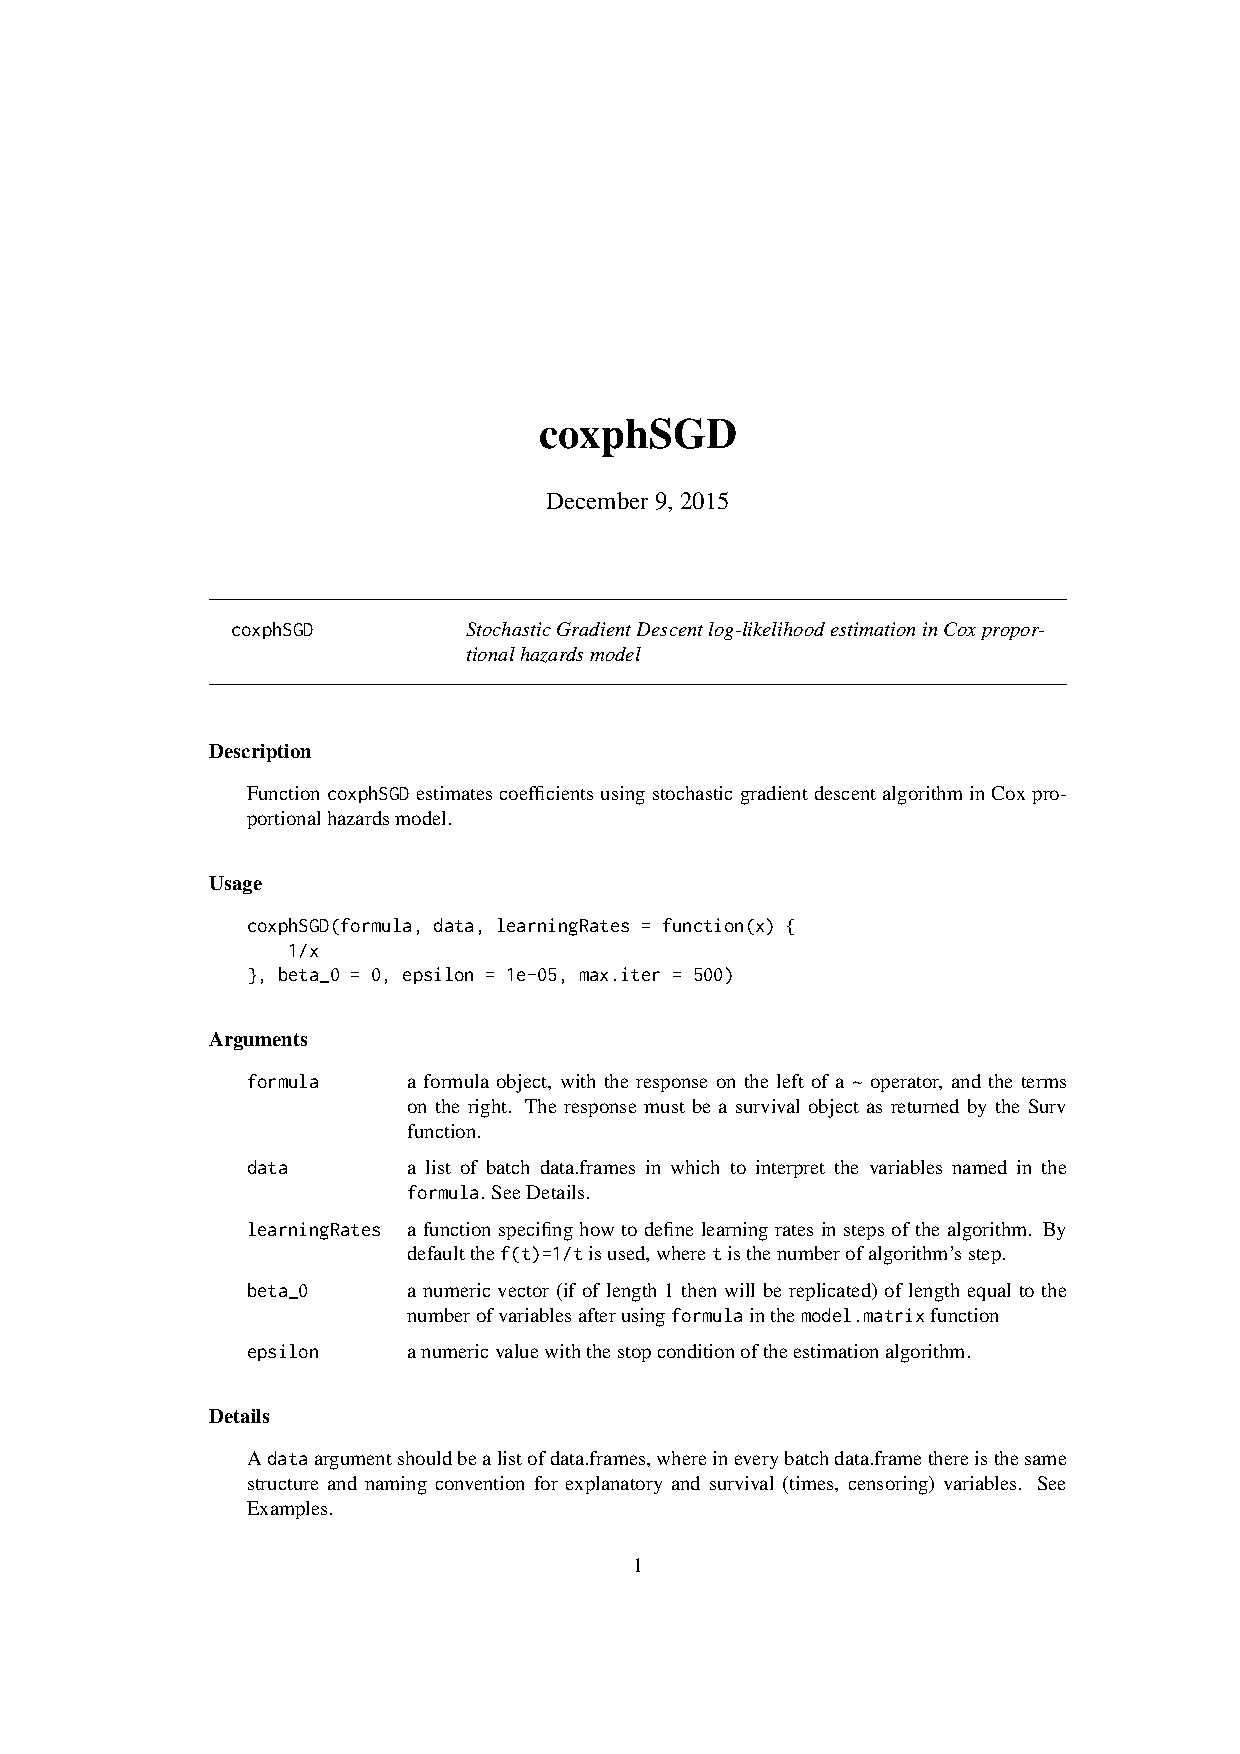
\includepdf[pages=-]{coxDoc8.pdf}
%\chapter{Dokumentacja pakietu RTCGA}
%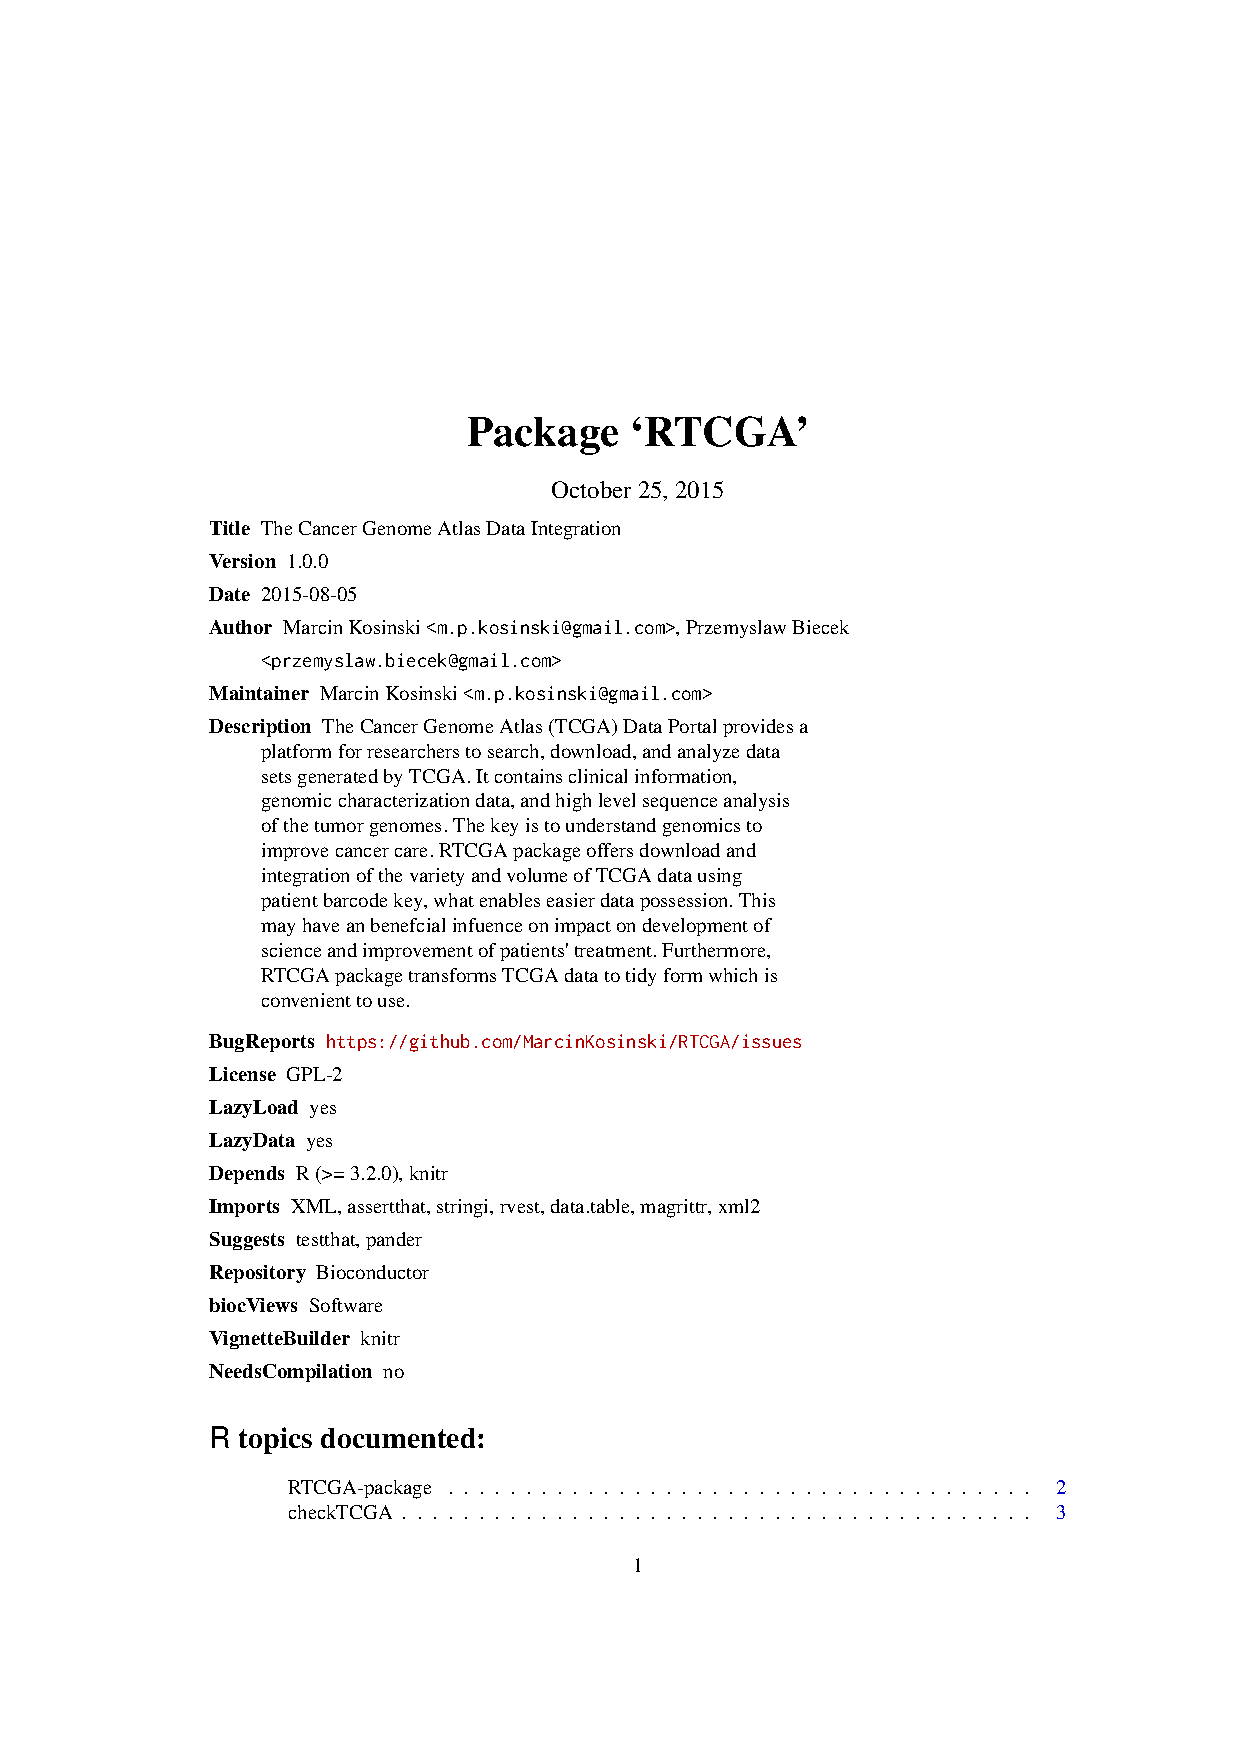
\includepdf[pages=-]{RTCGA.pdf}

\section{Analiza wpływu mutacji genów na czas życia}\label{dod:analiza}

\begin{Shaded}
\begin{Highlighting}[]
\NormalTok{extractSurvival <-}\StringTok{ }\NormalTok{function(cohorts)\{}
  
  \NormalTok{survivalData <-}\StringTok{ }\KeywordTok{list}\NormalTok{()}
  \NormalTok{for(i in cohorts)\{}
    \KeywordTok{get}\NormalTok{(}\KeywordTok{paste0}\NormalTok{(i, }\StringTok{".clinical"}\NormalTok{), }\DataTypeTok{envir =} \NormalTok{.GlobalEnv) %>%}
\StringTok{                }\KeywordTok{select}\NormalTok{(patient.bcr_patient_barcode,}
                             \NormalTok{patient.vital_status,}
                             \NormalTok{patient.days_to_last_followup,}
                             \NormalTok{patient.days_to_death ) %>%}
\StringTok{                }\KeywordTok{mutate}\NormalTok{(}\DataTypeTok{bcr_patient_barcode =} \KeywordTok{toupper}\NormalTok{(patient.bcr_patient_barcode),}
                       \DataTypeTok{patient.vital_status =} \KeywordTok{ifelse}\NormalTok{(patient.vital_status %>%}
\StringTok{                                                 }\KeywordTok{as.character}\NormalTok{() ==}\StringTok{"dead"}\NormalTok{,}\DecValTok{1}\NormalTok{,}\DecValTok{0}\NormalTok{),}
                   \DataTypeTok{barcode =} \NormalTok{patient.bcr_patient_barcode %>%}
\StringTok{                                     }\KeywordTok{as.character}\NormalTok{(),}
                 \DataTypeTok{times =} \KeywordTok{ifelse}\NormalTok{( !}\KeywordTok{is.na}\NormalTok{(patient.days_to_last_followup),}
                      \NormalTok{patient.days_to_last_followup %>%}
\StringTok{                        }\KeywordTok{as.character}\NormalTok{() %>%}
\StringTok{                        }\KeywordTok{as.numeric}\NormalTok{(),}
               \NormalTok{patient.days_to_death %>%}
\StringTok{                        }\KeywordTok{as.character}\NormalTok{() %>%}
\StringTok{                        }\KeywordTok{as.numeric}\NormalTok{() )}
                     \NormalTok{) %>%}
\StringTok{   }\KeywordTok{filter}\NormalTok{(!}\KeywordTok{is.na}\NormalTok{(times)) ->}\StringTok{ }\NormalTok{survivalData[[i]]}
  
  
  \NormalTok{\}}
  \KeywordTok{do.call}\NormalTok{(rbind,survivalData) %>%}
\StringTok{    }\KeywordTok{select}\NormalTok{(bcr_patient_barcode, patient.vital_status, times) %>%}
\StringTok{    }\NormalTok{unique  }

\NormalTok{\}}

\NormalTok{extractCohortIntersection <-}\StringTok{ }\NormalTok{function()\{}
  
  \KeywordTok{data}\NormalTok{(}\DataTypeTok{package =} \StringTok{"RTCGA.mutations"}\NormalTok{)$results[,}\DecValTok{3}\NormalTok{] %>%}
\StringTok{    }\KeywordTok{gsub}\NormalTok{(}\StringTok{".mutations"}\NormalTok{, }\StringTok{""}\NormalTok{, }\DataTypeTok{x =} \NormalTok{.) ->}\StringTok{ }\NormalTok{mutations_data}
  \KeywordTok{data}\NormalTok{(}\DataTypeTok{package =} \StringTok{"RTCGA.clinical"}\NormalTok{)$results[,}\DecValTok{3}\NormalTok{] %>%}
\StringTok{    }\KeywordTok{gsub}\NormalTok{(}\StringTok{".clinical"}\NormalTok{, }\StringTok{""}\NormalTok{, }\DataTypeTok{x =} \NormalTok{.) ->}\StringTok{ }\NormalTok{clinical_data}
  
  \KeywordTok{intersect}\NormalTok{(mutations_data, clinical_data)}
\NormalTok{\}}

\NormalTok{prepareForumlaSGD <-}\StringTok{ }\NormalTok{function(coxData)\{}
  \KeywordTok{as.formula}\NormalTok{(}\KeywordTok{paste}\NormalTok{(}\StringTok{"Surv(times, patient.vital_status) ~ "}\NormalTok{,}
                   \KeywordTok{paste}\NormalTok{(}\KeywordTok{names}\NormalTok{(coxData)[-}\KeywordTok{c}\NormalTok{(}\DecValTok{1092}\NormalTok{, }\DecValTok{1093}\NormalTok{)],}
                         \DataTypeTok{collapse=}\StringTok{"+"}\NormalTok{), }\DataTypeTok{collapse =} \StringTok{""}\NormalTok{))}
\NormalTok{\}}

\NormalTok{extractMutations <-}\StringTok{ }\NormalTok{function(cohorts, prc)\{}
  \NormalTok{mutationsData <-}\StringTok{ }\KeywordTok{list}\NormalTok{()}
  \NormalTok{for(i in cohorts)\{}
    \KeywordTok{get}\NormalTok{(}\KeywordTok{paste0}\NormalTok{(i, }\StringTok{".mutations"}\NormalTok{), }\DataTypeTok{envir =} \NormalTok{.GlobalEnv) %>%}
\StringTok{      }\KeywordTok{select}\NormalTok{(Hugo_Symbol, bcr_patient_barcode) %>%}
\StringTok{      }\KeywordTok{filter}\NormalTok{(}\KeywordTok{nchar}\NormalTok{(bcr_patient_barcode)==}\DecValTok{15}\NormalTok{) %>%}
\StringTok{      }\KeywordTok{filter}\NormalTok{(}\KeywordTok{substr}\NormalTok{(bcr_patient_barcode, }\DecValTok{14}\NormalTok{, }\DecValTok{15}\NormalTok{)==}\StringTok{"01"}\NormalTok{) %>%}
\StringTok{      }\NormalTok{unique ->}\StringTok{ }\NormalTok{mutationsData[[i]]}
  \NormalTok{\}}
  \KeywordTok{do.call}\NormalTok{(rbind,mutationsData) %>%}\StringTok{ }\NormalTok{unique ->}\StringTok{ }\NormalTok{mutationsData}
  \NormalTok{mutationsData %>%}
\StringTok{    }\KeywordTok{group_by}\NormalTok{(Hugo_Symbol) %>%}
\StringTok{    }\KeywordTok{summarise}\NormalTok{(}\DataTypeTok{count =} \KeywordTok{n}\NormalTok{()) %>%}
\StringTok{    }\KeywordTok{arrange}\NormalTok{(}\KeywordTok{desc}\NormalTok{(count)) %>%}
\StringTok{    }\KeywordTok{mutate}\NormalTok{(}\DataTypeTok{count_prc =} \NormalTok{count/}\KeywordTok{length}\NormalTok{(}\KeywordTok{unique}\NormalTok{(mutationsData$bcr_patient_barcode))) %>%}
\StringTok{    }\KeywordTok{filter_}\NormalTok{(}\KeywordTok{paste0}\NormalTok{(}\StringTok{"count_prc > "}\NormalTok{,prc)) %>%}
\StringTok{    }\KeywordTok{select}\NormalTok{(Hugo_Symbol) %>%}
\StringTok{    }\NormalTok{unlist ->}\StringTok{ }\NormalTok{topGenes}
  \NormalTok{mutationsData %>%}
\StringTok{    }\KeywordTok{filter}\NormalTok{(Hugo_Symbol %in%}\StringTok{ }\NormalTok{topGenes) ->}\StringTok{ }\NormalTok{mutationsData_top}
  \NormalTok{mutationsData_top %>%}
\StringTok{    }\NormalTok{dplyr::}\KeywordTok{group_by}\NormalTok{(bcr_patient_barcode) %>%}
\StringTok{    }\NormalTok{dplyr::}\KeywordTok{summarise}\NormalTok{(}\DataTypeTok{count =} \KeywordTok{n}\NormalTok{()) %>%}
\StringTok{    }\KeywordTok{group_by}\NormalTok{(count) %>%}\StringTok{ }
\StringTok{    }\KeywordTok{summarise}\NormalTok{(}\DataTypeTok{total =} \KeywordTok{n}\NormalTok{()) %>%}
\StringTok{    }\KeywordTok{arrange}\NormalTok{(}\KeywordTok{desc}\NormalTok{(count))}
  \KeywordTok{as.data.table}\NormalTok{(mutationsData_top) ->}\StringTok{ }\NormalTok{mutationsData_top_DT}
  \KeywordTok{dcast.data.table}\NormalTok{(mutationsData_top_DT, bcr_patient_barcode ~}\StringTok{ }\NormalTok{Hugo_Symbol, }\DataTypeTok{fill =} \DecValTok{0}\NormalTok{) %>%}
\StringTok{    }\NormalTok{as.data.frame ->}\StringTok{ }\NormalTok{mutationsData_top_dcasted}
  \NormalTok{mutationsData_top_dcasted[,-}\DecValTok{1}\NormalTok{][mutationsData_top_dcasted[,-}\DecValTok{1}\NormalTok{] !=}\StringTok{ "0"}\NormalTok{] <-}\StringTok{ }\DecValTok{1}
 \NormalTok{mutationsData_top_dcasted ->}\StringTok{ }\NormalTok{result}
  \KeywordTok{names}\NormalTok{(result) <-}\StringTok{ }\KeywordTok{gsub}\NormalTok{(}\KeywordTok{names}\NormalTok{(result),}\DataTypeTok{pattern =} \StringTok{"-"}\NormalTok{,  }\DataTypeTok{replacement =} \StringTok{""}\NormalTok{)}
  \NormalTok{result}
\NormalTok{\}}

\NormalTok{prepareCoxDataSplit <-}\StringTok{ }\NormalTok{function(mutationsData, survivalData, groups, }\DataTypeTok{seed =} \DecValTok{4561}\NormalTok{)\{}
  \NormalTok{mutationsData %>%}
\StringTok{  }\KeywordTok{mutate}\NormalTok{(}\DataTypeTok{bcr_patient_barcode =} \KeywordTok{substr}\NormalTok{(bcr_patient_barcode,}\DecValTok{1}\NormalTok{,}\DecValTok{12}\NormalTok{)) %>%}
\StringTok{  }\KeywordTok{left_join}\NormalTok{(survivalData,}
            \DataTypeTok{by =} \StringTok{"bcr_patient_barcode"}\NormalTok{) ->}\StringTok{ }\NormalTok{coxData}
  \NormalTok{coxData <-}\StringTok{ }\NormalTok{coxData[, -}\KeywordTok{c}\NormalTok{(}\DecValTok{1}\NormalTok{,}\DecValTok{2}\NormalTok{)]}
  \KeywordTok{apply}\NormalTok{(coxData[,-}\KeywordTok{c}\NormalTok{(}\DecValTok{1092}\NormalTok{, }\DecValTok{1093}\NormalTok{)], }\DataTypeTok{MARGIN =} \DecValTok{2}\NormalTok{,function(x)\{}
    \KeywordTok{as.numeric}\NormalTok{(}\KeywordTok{as.character}\NormalTok{(x))}
  \NormalTok{\}) ->}\StringTok{ }\NormalTok{coxData[,-}\KeywordTok{c}\NormalTok{(}\DecValTok{1092}\NormalTok{, }\DecValTok{1093}\NormalTok{)]}
  \KeywordTok{set.seed}\NormalTok{(seed)}
  \KeywordTok{sample}\NormalTok{(groups, }\DataTypeTok{replace =} \OtherTok{TRUE}\NormalTok{, }\DataTypeTok{size =} \DecValTok{6459}\NormalTok{) ->}\StringTok{ }\NormalTok{groups}
  \KeywordTok{split}\NormalTok{(coxData, groups) coxData_split}
\NormalTok{\}}
\end{Highlighting}
\end{Shaded}


\section{Implementacje optymalizacji w regresji logistycznej}\label{kody}
\begin{Shaded}
\begin{Highlighting}[]
\NormalTok{logitGD <-}\StringTok{ }\NormalTok{function(y, x, }\DataTypeTok{optim.method =} \StringTok{"GDI"}\NormalTok{, }\DataTypeTok{eps =} \FloatTok{10e-4}\NormalTok{,}
                    \DataTypeTok{max.iter =} \DecValTok{100}\NormalTok{, }\DataTypeTok{alpha =} \NormalTok{function(t)\{}\DecValTok{1}\NormalTok{/t\}, }\DataTypeTok{beta_0 =} \KeywordTok{c}\NormalTok{(}\DecValTok{0}\NormalTok{,}\DecValTok{0}\NormalTok{))\{}
  \KeywordTok{stopifnot}\NormalTok{(}\KeywordTok{length}\NormalTok{(y) ==}\StringTok{ }\KeywordTok{length}\NormalTok{(x) &}\StringTok{ }\NormalTok{optim.method %in%}\StringTok{ }\KeywordTok{c}\NormalTok{(}\StringTok{"GDI"}\NormalTok{, }\StringTok{"GDII"}\NormalTok{, }\StringTok{"SGDI"}\NormalTok{)}
            \NormalTok{&}\StringTok{ }\KeywordTok{is.numeric}\NormalTok{(}\KeywordTok{c}\NormalTok{(max.iter, eps, x)) &}\StringTok{ }\KeywordTok{all}\NormalTok{(}\KeywordTok{c}\NormalTok{(eps, max.iter) >}\StringTok{ }\DecValTok{0}\NormalTok{) &}
\StringTok{              }\KeywordTok{is.function}\NormalTok{(alpha))}
  \NormalTok{iter <-}\StringTok{ }\DecValTok{0}
  \NormalTok{err <-}\StringTok{ }\KeywordTok{list}\NormalTok{()}
  \NormalTok{err[[iter}\DecValTok{+1}\NormalTok{]] <-}\StringTok{ }\NormalTok{eps}\DecValTok{+1}
  \NormalTok{w_old <-}\StringTok{ }\NormalTok{beta_0}

  \NormalTok{res <-}\KeywordTok{list}\NormalTok{()}
  \NormalTok{while(iter <}\StringTok{ }\NormalTok{max.iter &&}\StringTok{ }\NormalTok{(}\KeywordTok{abs}\NormalTok{(err[[}\KeywordTok{ifelse}\NormalTok{(iter==}\DecValTok{0}\NormalTok{,}\DecValTok{1}\NormalTok{,iter)]]) >}\StringTok{ }\NormalTok{eps))\{}

    \NormalTok{iter <-}\StringTok{ }\NormalTok{iter +}\StringTok{ }\DecValTok{1}
    \NormalTok{if (optim.method ==}\StringTok{ "GDI"}\NormalTok{)\{}
      \NormalTok{w_new <-}\StringTok{ }\NormalTok{w_old +}\StringTok{ }\KeywordTok{alpha}\NormalTok{(iter)*}\KeywordTok{updateWeightsGDI}\NormalTok{(y, x, w_old)}
    \NormalTok{\}}
    \NormalTok{if (optim.method ==}\StringTok{ "GDII"}\NormalTok{)\{}
      \NormalTok{w_new <-}\StringTok{ }\NormalTok{w_old +}\StringTok{ }\KeywordTok{as.vector}\NormalTok{(}\KeywordTok{inverseHessianGDII}\NormalTok{(x, w_old)%*%}
\StringTok{                                   }\KeywordTok{updateWeightsGDI}\NormalTok{(y, x, w_old))}
    \NormalTok{\}}
    \NormalTok{if (optim.method ==}\StringTok{ "SGDI"}\NormalTok{)\{}
      \NormalTok{w_new <-}\StringTok{ }\NormalTok{w_old +}\StringTok{ }\KeywordTok{alpha}\NormalTok{(iter)*}\KeywordTok{updateWeightsSGDI}\NormalTok{(y[iter], x[iter], w_old)}
    \NormalTok{\}}
    \NormalTok{res[[iter]] <-}\StringTok{ }\NormalTok{w_new}
    \NormalTok{err[[iter]] <-}\StringTok{ }\KeywordTok{sqrt}\NormalTok{(}\KeywordTok{sum}\NormalTok{((w_new -}\StringTok{ }\NormalTok{w_old)^}\DecValTok{2}\NormalTok{))}

    \NormalTok{w_old <-}\StringTok{ }\NormalTok{w_new}

  \NormalTok{\}}
  \KeywordTok{return}\NormalTok{(}\KeywordTok{list}\NormalTok{(}\DataTypeTok{steps =} \KeywordTok{c}\NormalTok{(}\KeywordTok{list}\NormalTok{(beta_0),res), }\DataTypeTok{errors =} \KeywordTok{c}\NormalTok{(}\KeywordTok{list}\NormalTok{(}\KeywordTok{c}\NormalTok{(}\DecValTok{0}\NormalTok{,}\DecValTok{0}\NormalTok{)),err)))}
\NormalTok{\}}

\NormalTok{updateWeightsGDI <-}\StringTok{ }\NormalTok{function(y, x, w_old)\{}
  \CommentTok{#(1/length(y))*c(sum(y-p(w_old, x)), sum(x*(y-p(w_old, x))))}
  \KeywordTok{c}\NormalTok{(}\KeywordTok{sum}\NormalTok{(y-}\KeywordTok{p}\NormalTok{(w_old, x)), }\KeywordTok{sum}\NormalTok{(x*(y-}\KeywordTok{p}\NormalTok{(w_old, x))))}
\NormalTok{\}}

\NormalTok{updateWeightsSGDI <-}\StringTok{ }\NormalTok{function(y_i, x_i, w_old)\{}
  \KeywordTok{c}\NormalTok{(y_i-}\KeywordTok{p}\NormalTok{(w_old, x_i), x_i*(y_i-}\KeywordTok{p}\NormalTok{(w_old, x_i)))}
\NormalTok{\}}

\NormalTok{p <-}\StringTok{ }\NormalTok{function(w_old, x_i)\{}
  \DecValTok{1}\NormalTok{/(}\DecValTok{1}\NormalTok{+}\KeywordTok{exp}\NormalTok{(-w_old[}\DecValTok{1}\NormalTok{]-w_old[}\DecValTok{2}\NormalTok{]*x_i))}
\NormalTok{\}}




\NormalTok{inverseHessianGDII <-}\StringTok{ }\NormalTok{function(x, w_old)\{}
  \KeywordTok{solve}\NormalTok{(}
    \KeywordTok{matrix}\NormalTok{(}\KeywordTok{c}\NormalTok{(}
      \KeywordTok{sum}\NormalTok{(}\KeywordTok{p}\NormalTok{(w_old, x)*(}\DecValTok{1}\NormalTok{-}\KeywordTok{p}\NormalTok{(w_old, x))),}
      \KeywordTok{sum}\NormalTok{(x*}\KeywordTok{p}\NormalTok{(w_old, x)*(}\DecValTok{1}\NormalTok{-}\KeywordTok{p}\NormalTok{(w_old, x))),}
      \KeywordTok{sum}\NormalTok{(x*}\KeywordTok{p}\NormalTok{(w_old, x)*(}\DecValTok{1}\NormalTok{-}\KeywordTok{p}\NormalTok{(w_old, x))),}
      \KeywordTok{sum}\NormalTok{(x*x*}\KeywordTok{p}\NormalTok{(w_old, x)*(}\DecValTok{1}\NormalTok{-}\KeywordTok{p}\NormalTok{(w_old, x)))}
    \NormalTok{),}
    \DataTypeTok{nrow =}\DecValTok{2} \NormalTok{)}
  \NormalTok{)}
\NormalTok{\}}
\KeywordTok{set.seed}\NormalTok{(}\DecValTok{1283}\NormalTok{)}
\NormalTok{x <-}\StringTok{ }\KeywordTok{runif}\NormalTok{(}\DecValTok{10000}\NormalTok{)}
\NormalTok{z <-}\StringTok{ }\DecValTok{2} \NormalTok{+}\StringTok{ }\DecValTok{3}\NormalTok{*x}
\NormalTok{pr <-}\StringTok{ }\DecValTok{1}\NormalTok{/(}\DecValTok{1}\NormalTok{+}\KeywordTok{exp}\NormalTok{(-z))}
\NormalTok{y <-}\StringTok{ }\KeywordTok{rbinom}\NormalTok{(}\DecValTok{10000}\NormalTok{,}\DecValTok{1}\NormalTok{,pr)}


\NormalTok{global_loglog <-}\StringTok{ }\NormalTok{function(beta1, beta2, xX, yY)\{}
  \KeywordTok{sum}\NormalTok{(yY*(beta1+beta2*xX)-}\KeywordTok{log}\NormalTok{(}\DecValTok{1}\NormalTok{+}\KeywordTok{exp}\NormalTok{(beta1+beta2*xX)))}
\NormalTok{\}}



\NormalTok{calculate_outer <-}\StringTok{ }\NormalTok{function(x, y)\{}
  \NormalTok{## contours}
  \NormalTok{outer_res <-}\StringTok{ }\KeywordTok{outer}\NormalTok{(}\KeywordTok{seq}\NormalTok{(}\DecValTok{0}\NormalTok{,}\DecValTok{4}\NormalTok{, }\DataTypeTok{length =} \DecValTok{100}\NormalTok{),}
                     \KeywordTok{seq}\NormalTok{(}\DecValTok{0}\NormalTok{,}\DecValTok{5}\NormalTok{, }\DataTypeTok{length =} \DecValTok{100}\NormalTok{),}
                     \KeywordTok{Vectorize}\NormalTok{( function(beta1,beta2)\{}
                       \KeywordTok{global_loglog}\NormalTok{(beta1, beta2, }\DataTypeTok{xX =} \NormalTok{x, }\DataTypeTok{yY =} \NormalTok{y)}
                     \NormalTok{\} )}
  \NormalTok{)}

  \NormalTok{outer_res_melted <-}\StringTok{ }\KeywordTok{melt}\NormalTok{(outer_res)}


  \NormalTok{outer_res_melted$Var1 <-}\StringTok{ }\KeywordTok{as.factor}\NormalTok{(outer_res_melted$Var1)}
  \KeywordTok{levels}\NormalTok{(outer_res_melted$Var1) <-}\StringTok{ }\KeywordTok{as.character}\NormalTok{(}\KeywordTok{seq}\NormalTok{(}\DecValTok{0}\NormalTok{,}\DecValTok{4}\NormalTok{, }\DataTypeTok{length =} \DecValTok{100}\NormalTok{))}
  \NormalTok{outer_res_melted$Var2 <-}\StringTok{ }\KeywordTok{as.factor}\NormalTok{(outer_res_melted$Var2)}
  \KeywordTok{levels}\NormalTok{(outer_res_melted$Var2) <-}\StringTok{ }\KeywordTok{as.character}\NormalTok{(}\KeywordTok{seq}\NormalTok{(}\DecValTok{0}\NormalTok{,}\DecValTok{5}\NormalTok{, }\DataTypeTok{length =} \DecValTok{100}\NormalTok{))}
  \NormalTok{outer_res_melted$Var1 <-}\StringTok{ }\KeywordTok{as.numeric}\NormalTok{(}\KeywordTok{as.character}\NormalTok{(outer_res_melted$Var1))}
  \NormalTok{outer_res_melted$Var2 <-}\StringTok{ }\KeywordTok{as.numeric}\NormalTok{(}\KeywordTok{as.character}\NormalTok{(outer_res_melted$Var2))}
  \KeywordTok{return}\NormalTok{(outer_res_melted)}
\NormalTok{\}}



\KeywordTok{library}\NormalTok{(ggplot2); }\KeywordTok{library}\NormalTok{(ggthemes); }\KeywordTok{library}\NormalTok{(reshape2)}
\NormalTok{graphSGD <-}\StringTok{ }\NormalTok{function(beta, y, x, }\DataTypeTok{seed =} \DecValTok{4561}\NormalTok{, }\DataTypeTok{outerBounds =} \KeywordTok{calculate_outer}\NormalTok{(x,y))\{}
  \KeywordTok{set.seed}\NormalTok{(seed); }\NormalTok{beta <-}\StringTok{ }\KeywordTok{rev}\NormalTok{(beta); } \NormalTok{beta[}\DecValTok{2}\NormalTok{] ->}\StringTok{ }\NormalTok{XX; }\NormalTok{beta[}\DecValTok{1}\NormalTok{] ->}\StringTok{ }\NormalTok{YY}  
  \KeywordTok{logitGD}\NormalTok{(y, x, }\DataTypeTok{optim.method =} \StringTok{"GDI"}\NormalTok{,}\DataTypeTok{beta_0 =} \NormalTok{beta,}
          \DataTypeTok{eps =} \FloatTok{10e-4}\NormalTok{, }\DataTypeTok{max.iter =} \DecValTok{10000}\NormalTok{,}
          \DataTypeTok{alpha =} \NormalTok{function(t)\{}\DecValTok{1}\NormalTok{/(}\DecValTok{1000}\NormalTok{*}\KeywordTok{sqrt}\NormalTok{(t))\})$steps ->}\StringTok{ }\NormalTok{GDI.S}
  \KeywordTok{logitGD}\NormalTok{(y, x, }\DataTypeTok{optim.method =} \StringTok{"GDII"}\NormalTok{, }\DataTypeTok{beta_0 =} \NormalTok{beta,}
          \DataTypeTok{eps =} \FloatTok{10e-4}\NormalTok{, }\DataTypeTok{max.iter =} \DecValTok{5000}\NormalTok{)$steps ->}\StringTok{ }\NormalTok{GDII}
  \NormalTok{ind2 <-}\StringTok{ }\KeywordTok{sample}\NormalTok{(}\KeywordTok{length}\NormalTok{(y))}
  \KeywordTok{logitGD}\NormalTok{(y[ind2], x[ind2], }\DataTypeTok{optim.method =} \StringTok{"SGDI"}\NormalTok{, }\DataTypeTok{beta_0 =} \NormalTok{beta,}
          \DataTypeTok{max.iter =} \DecValTok{10000}\NormalTok{, }\DataTypeTok{eps =} \FloatTok{10e-4}\NormalTok{,}
          \DataTypeTok{alpha =} \NormalTok{function(t)\{}\DecValTok{1}\NormalTok{/}\KeywordTok{sqrt}\NormalTok{(t)\})$steps ->}\StringTok{ }\NormalTok{SGDI}\FloatTok{.1}\NormalTok{.S}
  \NormalTok{ind3 <-}\StringTok{ }\KeywordTok{sample}\NormalTok{(}\KeywordTok{length}\NormalTok{(y))}
  \KeywordTok{logitGD}\NormalTok{(y[ind3], x[ind3], }\DataTypeTok{optim.method =} \StringTok{"SGDI"}\NormalTok{, }\DataTypeTok{beta_0 =} \NormalTok{beta,}
          \DataTypeTok{max.iter =} \DecValTok{10000}\NormalTok{, }\DataTypeTok{eps =} \FloatTok{10e-4}\NormalTok{,}
          \DataTypeTok{alpha =} \NormalTok{function(t)\{}\DecValTok{5}\NormalTok{/}\KeywordTok{sqrt}\NormalTok{(t)\})$steps ->}\StringTok{ }\NormalTok{SGDI}\FloatTok{.5}\NormalTok{.S}
  \NormalTok{ind4 <-}\StringTok{ }\KeywordTok{sample}\NormalTok{(}\KeywordTok{length}\NormalTok{(y))}
  \KeywordTok{logitGD}\NormalTok{(y[ind4], x[ind4], }\DataTypeTok{optim.method =} \StringTok{"SGDI"}\NormalTok{, }\DataTypeTok{beta_0 =} \NormalTok{beta,}
          \DataTypeTok{max.iter =} \DecValTok{10000}\NormalTok{, }\DataTypeTok{eps =} \FloatTok{10e-4}\NormalTok{,}
          \DataTypeTok{alpha =} \NormalTok{function(t)\{}\DecValTok{6}\NormalTok{/}\KeywordTok{sqrt}\NormalTok{(t)\})$steps ->}\StringTok{ }\NormalTok{SGDI}\FloatTok{.6}\NormalTok{.S}
  \KeywordTok{do.call}\NormalTok{(rbind, }\KeywordTok{c}\NormalTok{(GDI.S, GDII, SGDI}\FloatTok{.1}\NormalTok{.S, SGDI}\FloatTok{.5}\NormalTok{.S, SGDI}\FloatTok{.6}\NormalTok{.S)) ->}\StringTok{ }\NormalTok{coeffs}
  \KeywordTok{unlist}\NormalTok{(}\KeywordTok{lapply}\NormalTok{(}\KeywordTok{list}\NormalTok{(GDI.S, GDII, SGDI}\FloatTok{.1}\NormalTok{.S, SGDI}\FloatTok{.5}\NormalTok{.S, SGDI}\FloatTok{.6}\NormalTok{.S),}
                \NormalTok{length)) ->}\StringTok{ }\NormalTok{algorithm}
  \NormalTok{data2viz <-}\StringTok{ }\KeywordTok{cbind}\NormalTok{(}\KeywordTok{as.data.frame}\NormalTok{(coeffs),}
  \DataTypeTok{algorithm =} \KeywordTok{unlist}\NormalTok{(}\KeywordTok{mapply}\NormalTok{(rep,}
                              \KeywordTok{c}\NormalTok{(}\KeywordTok{paste}\NormalTok{(}\StringTok{"GDI"}\NormalTok{, }\KeywordTok{length}\NormalTok{(GDI.S), }\StringTok{"steps"}\NormalTok{),}
                              \KeywordTok{paste}\NormalTok{(}\StringTok{"GDII"}\NormalTok{, }\KeywordTok{length}\NormalTok{(GDII), }\StringTok{"steps"}\NormalTok{),}
                              \KeywordTok{paste}\NormalTok{(}\StringTok{"SGDI.1"}\NormalTok{, }\KeywordTok{length}\NormalTok{(SGDI}\FloatTok{.1}\NormalTok{.S), }\StringTok{"steps"}\NormalTok{),}
                              \KeywordTok{paste}\NormalTok{(}\StringTok{"SGDI.5"}\NormalTok{, }\KeywordTok{length}\NormalTok{(SGDI}\FloatTok{.5}\NormalTok{.S), }\StringTok{"steps"}\NormalTok{),}
                              \KeywordTok{paste}\NormalTok{(}\StringTok{"SGDI.6"}\NormalTok{, }\KeywordTok{length}\NormalTok{(SGDI}\FloatTok{.6}\NormalTok{.S), }\StringTok{"steps"}\NormalTok{)),}
                            \NormalTok{algorithm)))}
  \KeywordTok{names}\NormalTok{(data2viz)[}\DecValTok{1}\NormalTok{:}\DecValTok{2}\NormalTok{] <-}\StringTok{ }\KeywordTok{c}\NormalTok{(}\StringTok{"Intercept"}\NormalTok{, }\StringTok{"X"}\NormalTok{)}
  \NormalTok{data2viz$algorithm <-}\StringTok{ }\KeywordTok{factor}\NormalTok{(data2viz$algorithm, }\DataTypeTok{levels =} \KeywordTok{rev}\NormalTok{(}\KeywordTok{levels}\NormalTok{(data2viz$algorithm)))}
  \KeywordTok{ggplot}\NormalTok{()+}
\StringTok{    }\KeywordTok{geom_path}\NormalTok{(}\KeywordTok{aes}\NormalTok{(}\DataTypeTok{x =} \NormalTok{data2viz$X,}
                  \DataTypeTok{y =} \NormalTok{data2viz$Intercept,}
                  \DataTypeTok{col =} \NormalTok{data2viz$algorithm,}
                  \DataTypeTok{group =} \NormalTok{data2viz$algorithm), }\DataTypeTok{size =} \DecValTok{1}\NormalTok{) +}
\StringTok{    }\KeywordTok{geom_point}\NormalTok{(}\KeywordTok{aes}\NormalTok{(}\KeywordTok{as.vector}\NormalTok{(}\KeywordTok{round}\NormalTok{(}\KeywordTok{coefficients}\NormalTok{(}\KeywordTok{glm}\NormalTok{(y~x,}
                          \DataTypeTok{family =} \StringTok{'binomial'}\NormalTok{)), }\DecValTok{2}\NormalTok{)[}\DecValTok{2}\NormalTok{]),}
                   \KeywordTok{as.vector}\NormalTok{(}\KeywordTok{round}\NormalTok{(}\KeywordTok{coefficients}\NormalTok{(}\KeywordTok{glm}\NormalTok{(y~x,}
                          \DataTypeTok{family =} \StringTok{'binomial'}\NormalTok{)), }\DecValTok{2}\NormalTok{)[}\DecValTok{1}\NormalTok{])),}
               \DataTypeTok{col =} \StringTok{"black"}\NormalTok{, }\DataTypeTok{size =} \DecValTok{4}\NormalTok{, }\DataTypeTok{shape =} \DecValTok{15}\NormalTok{) +}
\StringTok{    }\KeywordTok{geom_point}\NormalTok{(}\KeywordTok{aes}\NormalTok{(}\DataTypeTok{x=}\NormalTok{XX, }\DataTypeTok{y=}\NormalTok{YY),}
               \DataTypeTok{col =} \StringTok{"black"}\NormalTok{, }\DataTypeTok{size =} \DecValTok{4}\NormalTok{, }\DataTypeTok{shape =} \DecValTok{17}\NormalTok{) +}
\StringTok{    }\KeywordTok{theme_bw}\NormalTok{(}\DataTypeTok{base_size =} \DecValTok{20}\NormalTok{) +}
\StringTok{    }\KeywordTok{theme}\NormalTok{(}\DataTypeTok{panel.border =} \KeywordTok{element_blank}\NormalTok{(),}
          \DataTypeTok{legend.key =} \KeywordTok{element_blank}\NormalTok{()) +}
\StringTok{    }\KeywordTok{scale_colour_brewer}\NormalTok{(}\DataTypeTok{palette=}\StringTok{"Set1"}\NormalTok{, }\DataTypeTok{name =} \StringTok{'Algorithm'}\NormalTok{) +}
\StringTok{    }\KeywordTok{xlab}\NormalTok{(}\StringTok{'X'}\NormalTok{) +}\KeywordTok{ylab}\NormalTok{(}\StringTok{'Intercept'}\NormalTok{)}
\NormalTok{\}}
\end{Highlighting}
\end{Shaded}

\small\bibliography{biblioteczka}

%\begin{thebibliography}{99}

\bibitem[1]{aldrich1} Aldrich J., (1997) \textit{R. A. Fisher and the Making of Maximum Likelihood 1912 – 1922}, Statistical Science
1997, Vol. 12, No. 3, 162-176.

\bibitem[2]{assel} Asselain B., Mould R. F., (2010) \textit{Methodology of the Cox proportional hazards model},  Journal of Oncology 2010, volume 60, Number 5,  403–409.

\bibitem[3]{biecek1} Biecek P., (2011) \textit{Przewodnik po pakiecie R}, Rozprawa doktorska, Oficyna Wydawnicza GiS, wydanie II.

\bibitem[4]{bott1} Bottou L., (2010) \textit{Large-Scale Machine Learning with Stochastic Gradient Descent}.

\bibitem[5]{bottDOD} Bottou L., (1998), \textit{Online Learning and Stochastic
Approximations}.


\bibitem[6]{bott2} Bottou L., (2012) \textit{Stochastic Gradient Descent Tricks}.

\bibitem[7]{burzyk1} Burzykowski T., (2015?) \textit{Notatki do przedmiotu Biostatystyka}, \texttt{https://e.mini.pw.edu.pl/sites/default/files/biostatystyka.pdf}.

\bibitem[8]{cox0} Cox D. R. (1962) \textit{Renewal Theory. Methuen Monograph on Applied Probability
\& Statistics}, London: Methuen.

\bibitem[9]{cox}  Cox D. R., (1972) \textit{Regression models and life-tables (with discussion)}, Journal of the Royal Statistical Society Series B 34:187-220.. 

\bibitem[10]{dennis} Dennis J. E. Jr., Schnabel R. B., (1983), \textit{Numerical Methods For Un-
constrained Optimization and Nonlinear Equations}, Prentice-Hall.


\bibitem[11]{finkel}  Finkel J. R., Kleeman A., Manning C. D., (2008), \textit{Efficient, Feature-based, Conditional Random Field Parsing}, Proc. Annual Meeting of the ACL.

\bibitem[12]{fisher1} Fisher R. A., (1912) \textit{An absolute criterion for fitting frequency curves}. 

\bibitem[13]{fisher2} Fisher R. A., (1922) \textit{On the mathematical foundations of theoretical statistics}, Philos. Trans. Roy. Soc. London Ser. A 222 309-368.

\bibitem[14]{fortuna} Fortuna Z., Macukow B., Wąsowski J., (2006), \textit{Metody Numeryczne}, Wydawnictwa Naukowo-Techniczne.

\bibitem[15]{gauss1} Gauss C. F., (1809) \textit{Theoria Motus Corporum Coelestium}.

\bibitem[16]{gagol1} Gągolewski M., (2014) \textit{Programowanie w języku R}, Wydawnictwo Naukowe PWN.


\bibitem[17]{hald} Hald A., (1949) \textit{Maximum likelihood estimation of the parameters of a normal distribution which is truncated at a known point}, Skandinavisk Aktuarietidskrift, 119-134.

\bibitem[18]{hutch1} Hutchinson J. B., (1928) \textit{The Application of the "Method of Maximum Likelihood" to the Estimation of Linkage}, Genetics. 1929 Nov; 14(6): 519–537.


\bibitem[19]{kenward1} Kenward M. G., Lesaffre E. and Molenberghs G., (1994) \textit{An Application of Maximum Likelihood and Generalized Estimating Equations to the Analysis of Ordinal Data from a Longitudinal Study with Cases Missing at Random}, Biometrics
Vol. 50, No. 4 (Dec., 1994), pp. 945-953.

\bibitem[20]{kotlowski} Kotłowski W., (2012), Notatki do przedmiotu \textit{Techniki Optymalizacji} prowadzonego na Politechnice Poznańskiej, \\ \texttt{http://www.cs.put.poznan.pl/wkotlowski/teaching/wyklad3b.pdf}

\bibitem[21]{legendre1} Legendre A. M., (1804) \textit{Nouvelles m\`ethods pour la d\`etermination des orbites des com\`etes}.

\bibitem[22]{milewski} Milewski S., (2006) Konspekt do przedmiotu \textit{Metody Numeryczne} prowadzonego na Politechnice Krakowskiej, \\ \texttt{http://l5.pk.edu.pl/images/skrypty/Metody\_numeryczne\_1}

\bibitem[23]{millar1} Millar R. B., (2011) \textit{Maximum Likelihood Estimation and Inference: With Examples in R, SAS and ADMB, chapter 6. Some Widely Used Applications of Maximum Likelihood}, John Wiley \& Sons, Ltd.

\bibitem[24]{murata} Murata N., (1998), \textit{A Statistical Study of On-line Learning. In Online Learning
and Neural Networks}, Cambridge University Press.

\bibitem[25]{niemiro} Niemiro W., (2011) Skrypt do przedmiotu \textit{Statystyka} prowadzonego na Uniwersytecie Warszawskim, \\ \texttt{http://www-users.mat.umk.pl/$\sim$wniem/Statystyka/Statystyka.pdf}

\bibitem[26]{norwe} Norwegian Multicentre Study Group, (1981) \textit{Timolol-induced reduction in
mortality and reinfarction}, The New England  Journal of Medicine; 304: 801-7.


\bibitem[27]{mit0} Panchenko D., (2006), Notatki do otwartego kursu MIT \textit{Statistics for Applications, Lecture 2: Maximum Likelihood Estimators.}, \\
\texttt{http://ocw.mit.edu/courses/mathematics/18-443-statistics-for-applications-fall-2006/}



\bibitem[28]{mit1} Panchenko D., (2006), Notatki do otwartego kursu MIT \textit{Statistics for Applications, Lecture 3: Properties of MLE: consistency, asymptotic normality. Fisher information.}, \\
\texttt{http://ocw.mit.edu/courses/mathematics/18-443-statistics-for-applications-fall-2006/}



\bibitem[29]{programikr} R Core Team, (2013) \textit{R: A language and environment for statistical computing.} R Foundation for Statistical Computing, Wiedeń , ISBN 3-900051-07-0, \texttt{http://www.R-project.org/}.


\bibitem[30]{robbins} Robbins H. E., Siegmund. D. O., (1971), \textit{A convergence theorem for non negative almost supermartingales
and some applications}, In Proc. Sympos. Optimizing
Methods in Statistics, pages 233–257, Ohio State
University. Academic Press, New York.

\bibitem[31]{rydl1} Rydlewski J., (2009) \textit{Estymatory Największej Wiarogodności w Uogólnionych Modelach Regresji Nieliniowej}, Rozprawa doktorska.

\bibitem[32]{sokol} Sokołowski A., (2010) \textit{Jak rozumieć i wykonywać analizę przeżycia} \textit{http://www.statsoft.pl/Portals/0/Downloads/Jak\_rozumiec\_i\_wykonac\_analize\_przezycia.pdf}

\bibitem[33]{views} Statistics Views, (2014) \textit{ "I would like to think of myself as a scientist, who happens largely to specialise in the use of statistics"– An interview with Sir David Cox}. 

\bibitem[34]{ther} Therneau T. M., Grambsch P. M., (2000), \textit{Modeling Survival Data: Extending the Cox Model}, Springer.

\bibitem[35]{ADALINE} Widrow B, (1960), \textit{An adaptive "ADALINE" neuron using chemical "memistors"}, Technical Report No. 1553-2, Stanford University.

\bibitem[36]{widrow2} Widrow B, Stearns S. D., (1985), \textit{Adaptive Signal Processing, Prentice Hall}.

\bibitem[37]{wiki1} Wikipedia, encyklopedia wolnego dostępu \texttt{wikipedia.pl}
 
 \bibitem[38]{sfu1} Woodcock S, (2014), Notatki do otwartego kursu Uniwersytetu Simona Frasera \textit{ECON 837, Lecture 11 Asymptotic Properties of Maximum Likelihood Estimators}, \\ \texttt{http://www.sfu.ca/~swoodcoc/teaching/sp2014/econ837/11.mle.pdf}
 
\bibitem[39]{zieli} Zieliński R., (1990) \textit{Siedem wykładów wprowadzających do statystyki matematycznej}, Warszawa, Wydawnictwo Naukowe PWN.


\end{thebibliography}


\makestatement
\end{document}
